\documentclass[a4paper,twoside,12pt]{book}
\usepackage[utf8]{inputenc}
\usepackage{listings}
\usepackage{amsmath}
\usepackage{amsthm}
\usepackage{amsfonts}
\usepackage{amssymb}
\usepackage[english]{babel}
\usepackage[a4paper]{geometry}
\usepackage{graphicx}
\usepackage{epigraph}
\usepackage{color,psfrag}
\usepackage{fancyhdr}
\usepackage{makeidx}
\usepackage{mathpazo}
\usepackage{mathrsfs}
\usepackage{float}
\usepackage{datetime}
\usepackage{titlesec}
\usepackage{datetime}
\usepackage{afterpage}
\usepackage{pdflscape}
\usepackage{ragged2e}
\usepackage{adjustbox}
\usepackage{algorithm}%new
\usepackage{tcolorbox}
% \usepackage{algorithmicx}%new
\usepackage[noend]{algpseudocode}%new
\sloppy

%\usepackage{hyperref}
%\usepackage[numbers]{natbib}
\usepackage[labelfont=bf,textfont=it,labelsep=period,width=\textwidth]{caption}
\usepackage[unicode,pdfstartview={XYZ null null 1},pdfview={XYZ null null 1},pdfpagemode=UseOutlines]{hyperref}
\usepackage{booktabs}
\usepackage{graphicx}
\newcommand{\ra}[1]{\renewcommand{\arraystretch}{#1}}
\newcommand\blankpage{%
\null
\thispagestyle{empty}%
\addtocounter{page}{-1}%
\newpage}
\newdateformat{monthyeardate}{%
\monthname[\THEMONTH], \THEYEAR}


% \definecolor{szin}{rgb}{0.679,0.19,0.21} % Original color
\definecolor{szin}{rgb}{0.5, 0.62, 0.66}
\definecolor{szin2}{rgb}{0,0.445,0.734}
\definecolor{szin3}{rgb}{0,0.5,0}

\makeatletter
\let\stdl@chapter\l@chapter
\renewcommand*{\l@chapter}[2]{%
  \stdl@chapter{\textcolor{szin}{#1}}{\textcolor{szin}{#2}}}
\makeatother

%fejlï¿œc
\pagestyle{fancy}
\setlength{\headheight}{15.71667pt}
\lhead{\nouppercase{\rightmark}}
%\rhead{\nouppercase{\leftmark}}
\fancyhead[LE,RO]{\thepage}
\fancyfoot{}

%margomï¿œretek
\setlength{\marginparwidth}{0pt}
\setlength{\marginparsep}{0pt}
\setlength{\marginparpush}{0pt}
\setlength{\oddsidemargin}{24.1pt}
\setlength{\evensidemargin}{1pt}
\setlength{\footskip}{20pt}
\setlength{\headheight}{27.5pt}
    
%chapterstyles
\newcommand{\PreContentTitleFormat}{\titleformat{\chapter}[display]{\scshape\Large}
{\Large\filleft\MakeUppercase{\chaptertitlename} \Huge\thechapter}
{1ex}
{}
[\vspace{1ex}\titlerule]}
\newcommand{\ContentTitleFormat}{\titleformat{\chapter}[display]{\scshape\color{black}\huge}
{\color{szin}\Large\filleft\MakeUppercase{\chaptertitlename} \Huge\thechapter}
{1ex}
{\titlerule\vspace{1ex}\filright}
[\vspace{1ex}\titlerule]}
\newcommand{\PostContentTitleFormat}{\PreContentTitleFormat}
\PreContentTitleFormat


\begin{document}

\begin{titlepage}
	\begin{center}

		\textbf{\LARGE{Multilayer network analysis of sustainable, multimodal urban transport networks}}\\[3.3cm] %

		
\includegraphics[width=3.45cm,height=2.3cm]{images/ceulogo.eps}\\[3.4cm]
		{\Large{\textbf{Luis Guillermo Natera Orozco}}}\\[0.4cm]

		\medskip

		Department of Network and Data Science \\
		Central European University\\ [1.2cm]

		Supervisor: Federico Battiston \\
		External Supervisor: Michael Szell

		\vfill

		A Dissertation Submitted in Partial Fulfillment of the Requirements\\ for the Degree of Doctor of Philosophy in Network Science\\[2cm]

		%
\includegraphics[width=3cm,height=2cm]{images/ceulogo.eps}\\[0.5cm]
		% Central European University\\
		% Budapest, Hungary

		\vspace{1.0cm}
		\the\year
	\end{center}
\end{titlepage}

\newpage

\pagestyle{empty}

\mbox{}

\vfill

\noindent Luis Guillermo Natera Orozco\\
\emph{Multilayer network analysis of sustainable, multimodal urban transport networks}\\ 
\copyright \, \the\year 
\\ All rights reserved.



\mbox{}

\pagestyle{empty}

\newpage

\chapter*{Researcher declaration}
I Luis Guillermo Natera Orozco certify that I am the author of the work Multilayer network analysis of sustainable multimodal urban transport networks. I certify that this is solely my own original work, other than where I have clearly indicated, in this declaration and in the thesis, the contributions of others. The thesis contains no materials accepted for any other degrees in any other institutions.  The copyright of this work rests with its author. Quotation from it is permitted, provided that full acknowledgement is made. This work may not be reproduced without my prior written consent.

\subsection*{Statement of inclusion of joint work}
I confirm that Chapter~\ref{ch:litReview} is based on the paper ``Multimodal urban mobility and multilayer transport networks'', under review at \textit{Transport Reviews} which was written in collaboration with Laura Alessandretti, Meead Saberi, Michael Szell and Federico Battiston. Dr. Battiston and I conceived the idea of doing a review about the application of multiplex networks to the study of urban mobility systems. All authors contributed to the writing of the paper. Dr. Battiston endorses this statement with his signature below.

\vspace{.2cm}

I confirm that Chapter~\ref{ch:OverlapCensus} is based on the paper ``Extracting the multimodal fingerprint of urban transportation networks'', published in \textit{Findings}, the paper was written in collaboration with Federico Battiston, Gerardo I\~niguez, and Michael Szell. I, with Dr. Battiston and Dr. Szell conceived the idea of the overlap census. I collected the data and carried out the analyses. All authors developed the methods used, contributed to the writing of the paper on which the chapter is based and gave final approval for publication. Dr. Szell endorses this statement with his signature below.

\vspace{.2cm}

I confirm that Chapter~\ref{ch:BikeGrowth} is based on the paper ``Data-driven strategies for optimal bicycle network growth'', published in \textit{Royal Society Open Science}, the paper was written in collaboration with Federico Battiston, Gerardo I\~niguez, and Michael Szell. I, with Dr. Battiston and Dr. Szell conceived the research. I collected, processed and cleaned data, and carried out the computational analysis. All authors designed the algorithms, analysed the data and results, and helped draft the manuscript. Dr. Szell endorses this statement with his signature below.

\vspace{.2cm}

\noindent
I confirm that Chapter~\ref{ch:LQI} is based on the paper ``Quantifying life quality as walkability on urban networks: The case of Budapest'', published in \textit{International Conference on Complex Networks and Their Applications 2019}, the paper was written in collaboration with D\'avid Deritei, Anna Vancs\'o, and Orsolya V\'as\'arhelyi. I with Dr. Deritei and Dr. V\'as\'arhelyi conceived the research and methodology, all authors collected, processed and cleaned data, and carried out the computational analysis. Together with Dr. Deritei and Dr. V\'as\'arhelyi we analysed the results. All author helped draft the manuscript and gave final approval for its publication. Dr. V\'as\'arhelyi endorses this statement with her signature below.

\vspace{1.5cm}
\noindent
Signature of PhD Candidate:

\vspace{2cm}
\noindent
\monthyeardate\today


\vspace{3.5cm}
\noindent
Signature of Dr. Federico Battiston, endorsing statement of joint work:

\vspace{2cm}
\noindent
\monthyeardate\today


\vspace{3.5cm}
\noindent
Signature of Dr. Michael Szell, endorsing statement of joint work:

\vspace{2cm}
\noindent
\monthyeardate\today

\vspace{3.5cm}
\noindent
Signature of Dr. Orsolya V\'as\'arhelyi , endorsing statement of joint work:

\vspace{2cm}
\noindent
\monthyeardate\today




\chapter*{Abstract}
With more than half of the world's population living in cities, it is fundamentally important to understand how the complex system of urban mobility infrastructure, from sidewalks and bicycle paths to streets and rails, shapes and modifies human mobility. In this thesis, we use network science to study cities and their mobility infrastructures. We treat these infrastructures as layers of a multiplex network, such as sidewalks, bicycle paths, subway systems and streets, and develop and apply network science based tools to study these layers both individually and jointly. First, we survey the existing literature of cities as multiplex networks, from infrastructure and dynamics to existing measures, data and analysis tools. Second, we propose a new method to extract the multimodal profile from a city's multiplex transport network. We show how this method can be applied to identify multimodal similarities between cities. Third, we focus on the bicycle layer of the multimodal network, investigate its structure, and find that it consists of hundreds of disconnected patches. To connect these patches, we develop and apply data-driven, algorithmic network growth strategies, showing that small but focused investments allow to significantly increase the connectedness and directness of urban bicycle networks. In the fourth chapter, we present a data-driven, network-based method to quantify the livability of a city, computing pedestrian accessibility to amenities and services, taking into consideration safety and environmental variables. Finally, we discuss the main contributions of this thesis and outline possible applications and open questions for the future. We anticipate that this work contributes directly to the understanding of urban systems providing new insights and tools for the evaluation of sustainable urban mobility infrastructures. Understanding, improving, and evaluating urban mobility infrastructures are major steps for improving urban life and to plan ahead of climate change, thus a well-defined set of tools and metrics will be relevant to move forward.

\thispagestyle{empty}
% this is new:
% \newpage
% \newpage
% \chapter*{}

\newpage
\frontmatter
\begin{center}
    \thispagestyle{empty}
    \vspace*{\fill}
	\begin{flushright}
    To Pau. \\
	We did it.
	\end{flushright}
    \vspace*{\fill}
\end{center}
\thispagestyle{empty}
% this ends new

% this is new:
\newpage
\frontmatter
\epigraph{hablo de la ciudad, pastora de siglos, madre que nos engendra y nos devora, nos inventa y nos olvida.}{Octavio Paz\\ \textit{Hablo de la ciudad} (1986)}
\vfill
\thispagestyle{empty}
% this ends new

\chapter*{Acknowledgements}
The entire process of a doctoral program and dissertation involves an incredible support network. I would like to thank and acknowledge several people that have, whether realizing it or not, influenced this work. First, I would like to express my gratitude to my advisors Michaell Szell and Federico Battiston, for their tireless, caring support in this endeavor. Their guidance has been invaluable. I thank Gerardo I\~niguez for his contributions, guidance, and support.

I thank my friends and colleagues from the Department of Network and Data Science: J\'ulia Perczel, Orsolya V\'as\'arhelyi, D\'avid Deritei, Rebeka O. Szab\'o, Matteo Neri, Manran Zhu, Milan Janosov for their friendship and support during the Ph.D. They, along with the rest of the department, including Olga Peredi, the other Ph.D. students, faculty, postdocs, and visitors, provided a fun and stimulating environment. Special thanks to Agnes Toth from the Center for Academic Writing for her insightful comments.

My appreciation goes to my former mentors who set me on this path: Rosy Laguna, for planting the seed to view the world through numbers. Sandra Vald\'es, Pedro Alcocer, and Alfredo Hidalgo for setting me on a path to understand, plan and build better cities. Rossana Reguillo, thank you for helping me have my first steps into academic research.

I thank all my friends for your kind encouragement, patience, and support. It was essential to keep me sane during the last four years. Thank you, Jorge, Susana, Juan Carlos, Alejandro, Diana, Pily, Gabriel, Andrea, Andr\'es, Gaby, Juan Carlos, Javier, Ana, Juan Carlos, Juan Pablo, Luc\'ia, Alfredo, Alexa, Carlos, H\'ector and to the many, many others that have been there for me when needed. Thank you for your friendship.

I am fortunate to have two families supporting and rooting for me. I thank the Velasco Salcedo's, Gaby, Andrea, Gaby, and  Guillermo, for their unconditional love and support. To the Natera Orozco's, my parents, Lupita y Jaime, my brother, Jorge — you have provided me with incredible support, endless encouragement, and love. Gracias.

Most importantly, I want to thank Pau. She alone knows what went into this Ph.D. and thesis. How the road was, the lows and highs, the bumps along the road. This has been a shared journey. Her support, encouragement, and love have been essential to be here today. Pau — Thank you for this amazing ride that is life with you. I love you. This thesis is for you.

\newpage



\thispagestyle{empty}

\newpage
\frontmatter

\pagestyle{fancy}

\newpage
\addcontentsline{toc}{chapter}{Contents}

\PreContentTitleFormat

\def\luis#1{{\small\color{red}\textbf{[Luis: #1]}}}

\tableofcontents

\PreContentTitleFormat

\newpage

\PreContentTitleFormat

\pagestyle{fancy}

\newpage
\PreContentTitleFormat
\pagestyle{fancy}

% \listoftables
% \addcontentsline{toc}{chapter}{List of Tables}

% \listoffigures
% \addcontentsline{toc}{chapter}{List of Figures}

\PreContentTitleFormat
\newpage
\mainmatter
\ContentTitleFormat

\chapter{Introduction: Cities and networks}
%Why study cities? 

\epigraph{Cities have the capability of providing something for everybody, only because, and only when, they are created by everybody.}{Jane Jacobs, \textit{The Death and Life of Great American Cities} (1961, p. 238)}

As a complex system, a city offers a fertile study ground from multiple perspectives. Urban studies, from sociological perspectives to more technical ones such as engineering, have engaged in analyzing different aspects of urban life. Due to this diversity and overlapping approaches, the ``science of cities'' is inherently interdisciplinary.

\section{From architecture to network science, a personal journey}

As an architect my first approach to study cities was from the buildings perspective, understanding how, by building, we delimit and shape spaces that model experiences in the city~\cite{gehl1971life}. These buildings are fundamental to define public spaces, mobility infrastructures, and even services that enable us to inhabit the \textit{ville}~\cite{sennett2018building}. The way we shape the city has an influence in how we inhabit it. Thus, understanding its infrastructures is fundamental to understand and plan better cities for an increasingly complex future. Especially, when tackling urban mobility challenges, the way we plan, build and use mobility infrastructures is fundamentally entangled with the livability of our cities.

%Talk about curiosity, why study cities from the complex systems perspective, and specially from network science.
After working in designing public policies to promote bicycle infrastructure in my home-city's government, I became interested in getting to understand the relation between different transportation modes, and how cities and their mobility infrastructures could be studied using large scale data in a systematic way. This curiosity led me to the complex systems field, and the use of network science to study cities.

\luis{write more about moving between architeture and network science.}
\begin{itemize}
    \item Public spaces
    \item Urban mobility
    \item Complexity, cities as fractals (Batty)
    \item The always evolving city. We cannot predict the future, we can build it. Tools to understand the present and build a sustainable future.
    \item Personal reflection of interdisciplinary approaches (social sciences benefit from quantitative methods, but it is important to acknowledge interdisciplinary as a two way street, recognize the importance of social sciences, and the long tradition of urban studies. Not because we have a hammer, should we treat everything as if it were a nail) \luis{This idea might go to conclusions}
\end{itemize}
% While predicting how the future city will be is an impossible task, understanding how it has evolve and what is its state of development is possible. This understanding 


\section{Aim and structure of the thesis}

\luis{I still have to write about the thesis, from where does it start (complex systems and the study of cities) to the main contributions. I anticipate two paragraphs for the complex systems and cities, and two more paragraphs for the contributions/overview.}

The primary aim of this thesis is to contribute to the better understanding of the structural properties of multimodal transportation networks in urban areas. For that, we build on the tools and methods of network science to analyze the underlying complexity of urban mobility infrastructure. 

In the first part of this thesis we focus the attention on the multimodal infrastructure networks, first providing a review of previous works, and then giving an original contribution to the analysis of multilayer transportation networks. In the second part of the thesis we focus the attention to specific layers, first bicycle, then pedestrian infrastructure.

This thesis is structured as follows:

\begin{itemize}
    \item Chapter~\ref{ch:litReview}: We provide a review of previous works on multimodal transportation and mobility research from a complex systems' perspective. First we focus on the infrastructure and measures to quantify it, then on the mobility dynamics on top of these infrastructures, and finally we offer a review of available datasets and tools to analyze this specific type of networks.
    \item Chapter~\ref{ch:OverlapCensus}: We make an original contribution to the field by proposing a method to extract the multimodal profile from a city's multiplex transport network. We apply our methods to fifteen cities, finding clusters of cities with similar multimodal infrastructure.
    \item Chapter~\ref{ch:BikeGrowth}: We focus our attention in the bicycle layer of the multimodal network and propose algorithmic approaches to improve its connectivity. We find that focalized investment has the potential to rapidly improve the connectedness and directness of the bicycle infrastructure.
    \item Chapter~\ref{ch:LQI}: We present a methodology to measure the quality of life in a city based on the pedestrian accessibility to amenities and services. We apply the methodology to Budapest and show how it can be used to capture inequalities in neighborhoods. 
    \item Chapter~\ref{ch:Conclusion}: We review the main contributions from this thesis, and outline future streams of work and open questions. 
\end{itemize}\pagestyle{fancy} %Introduction
\chapter{Related Work}\label{ch:litReview}

The primary aim of this section is to offer a comprehensive review of multimodal transportation and mobility research focusing on recent complex systems approaches. In such approaches, the city is studied as a complex system \cite{batty2013new,lobo2020urban}, in which especially urban transport infrastructure, such as streets, sidewalks, bicycle lanes and public transportation systems can be well modelled and understood using methods from network science. From this perspective, single-layer spatial networks, especially transportation networks, have been widely studied~\cite{lin2013complex,barthelemy2011spatial,ding2019application}, finding different topological properties~\cite{jiang2004topological,cardillo2006structural,barthelemy2008patterns,batty2008size,barthelemy2011spatial,strano2013comparative,louf2014typology,boeing2020multiscale}, distribution of centrality metrics~\cite{crucitti2008centrality,boeing2018planarity,kirkley2018structural}, and network growth processes~\cite{makse1995growth,strano2012evolution}. Further topics studied include impacts of the street networks on pedestrian volume \cite{hajrasouliha2015connectivity}, accessibility and vitality of cities~\cite{denadai2016death,biazzo2019accesibility,natera2019walkability}, and resilience and growth of different transportation networks~\cite{baggag2018resilience,ferretti2019resilience,natera2020growth}. %Despite the many successes, network science should be applied to transportation systems with care \cite{zanin2018studying}. 

The most recent of these approaches can be seen as the beginning of the emerging field of Urban Data Science, which exploits large-scale new urban data sets with tools combining geoinformatics, data and network science \cite{organizers2019roundtable,resch2019hds}.

In this section we focus on the combined use of single-layer networks as multilayer networks to characterize the multimodal transportation infrastructure of cities and the human mobility taking place on them. We follow the primal approach to networks \cite{porta2006primal}, where streets and mobility infrastructure constitute the network links, and intersections (bus stops, subway stations, etc.) constitute the nodes of the network.

The remainder of this section is arranged as follows. Section~\ref{sec:multilayernetworks} introduces the mathematical concept of multilayer networks and related theoretical research underlying network science approaches to the topic. In Section~\ref{sec:multimodalinfrastructures} we cover urban infrastructures, measures to quantify their multimodality and models to reproduce the interconnected structures of real-world transportation systems. In Section~\ref{sec:multimodalmobility} we focus on mobility, flows and navigation across these multimodal systems, and implications for transportation choices. %In Section ~\ref{sec:datatools} we cover the relevant open datasets and the main software tools which can be used to analyse multimodal transportation systems. We conclude with an outlook and a summary of open questions for the research community in Section~\ref{sec:conclusions}. 

\section{Multilayer networks: a framework for multimodality}\label{sec:multilayernetworks}

Over the last decades, networks have emerged as a versatile tool to understand, map and visualise the interconnected architecture of a wide range of complex systems~\cite{albert2002statistical,dorogovtsev2002evolution, newman2003structure, boccaletti2006complex}, in particular spatially-embedded ones~\cite{barthelemy2011spatial}. Formally, a network -- or graph -- $\mathcal G = (\mathcal N, \mathcal L)$ consists of a set of nodes $\mathcal N$, and a second set $\mathcal L$ of edges, describing connections among unordered pairs of elements of the first set. This information can be conveniently stored into an adjacency matrix ${A=a_{ij}}$, where $i=1, \dots, N$ are the nodes, and $a_{ij}=1$ if there is a link between nodes $i$ and $j$, $a_{ij}=0$ if there is no link between $i$ and $j$. In transportation systems~\cite{lin2013complex}, nodes can represent the stations of a network, and links direct connections between them. The adjacency matrix can also include weights $W=w_{ij}$, where $w_{ij}$ are positive real numbers, for instance describing how strongly connected two nodes are. For spatial systems, weights are often taken as the reciprocal of the distance between two nodes, or the time it takes to travel from one to another, i.e. $w_{ij}=1/d_{ij}$ or $w_{ij}=1/t_{ij}$.

More recently, network scientists have put a lot of effort in characterising the structure of systems which are formed by different interconnected networks. Also widespread in social and biological networks, these structures are natural for transportation systems. Think for instance of the largest transportation hubs in worldwide cities, where stations are routinely served by bus, underground and railway infrastructures.

Indeed, most urban transportation systems systemically rely on the interplay between different mean of transportation. These systems can be conveniently described by \textit{multiplex} or \textit{multilayer} networks. Here we introduce the so-called \textit{vectorial} formalism for multilayer networks~\cite{boccaletti2014structure, battiston2014structural}, widely used in most papers on multimodal transportation. We note that an alternative description can be provided by a more mathematically involved \textit{tensorial} framework~\cite{dedomenico2013mathematical, kivela2014multilayer}.  

In multilayer networks, links of different types, describing for instance a different mean of transportation, are embedded into different \textit{layers}. Each layer $\alpha$, $\alpha = 1, \ldots, M$, is described by an adjacency matrix 
$ W^{[\alpha]} = w_{ij}^{[\alpha]}$. In a multimodal urban transportation networks with three layers, $\alpha=1$ can represent the bus network, $\alpha=2$ the underground network, and $\alpha=3$ the urban railway network. The full transportation system $\mathcal M$ can be described as $\mathcal W = \{W^{[1]}, \ldots,  W^{[M]}\}$. Nodes $i=1, \dots, N$ are labeled in the same order in all networks. 

In the case of transportation networks, identifying nodes of different networks (urban location) as the same station might not provide the most complete description of the multimodal network. Think for instance of the largest stations in mega-cities, like King's Cross - St. Pancras in London, Grand Central Station in New York or Hongqiao transportation hub in Shanghai. All of those are identified by a unique location (node index) $i$ across the different transportation layers. However, sometimes switching from one mean of transportation to another within the same station might require a non negligible fraction of time and effort, given the complexity and size of the overall infrastructure. 

For this reason, it is often relevant to complement the description of the \textit{intra-layer} connections present in the system, with \textit{inter-layer} links associated to the cost, physical distance or time required to switch layers. Inter-layer links between layers $\alpha$ and $\beta$ at a node $i$ can be encoded through the inter-layer matrix $C_i=c_i^{[\alpha \beta]}$, and all such inter-layer connections can be stored in the vector $ C = \{C_1, \ldots, C_N\}$. In this case, the full multiplex structure of the system is described by taking into account both intra-layer and inter-layer connectivity, hence $\mathcal M = (W,  C)$. Inter-links may be neglected for many measures focusing on diversity~\cite{battiston2014structural}, as well as correlations~\cite{nicosia2015measuring} across the layers of the systems, relevant to assess the different roles and geographical spanning of the different mean of transportations of a multilayer network. 

Multilayer networks are a natural framework for multimodal networks. Indeed, one of the pioneering works introducing the framework and concept of `layered complex networks'~\cite{kurant2006layered} explicitly focused on the case of transportation systems, where a first layer encoded the physical infrastructure of the system, and the second one described the flows on such infrastructure. Other early works on the topic also dealt with interconnected systems at the wordwide level, focusing on different modes of transport such as the multiplex airline networks~\cite{cardillo2013emergence}.

Noticeably, multimodal infrastructures seem to possess exclusive characteristics, different from other multilayer networks. For instance, when tools to assess the redundancy of the different layers are considered, transportation networks are often found to be irreducible~\cite{dedomenico2015structural}. Differently from many biological systems, where layers often duplicate information to guarantee the interconnected system a high level of robustness, the layers of a multiplex transportation systems are purposedly engineered to be different, in order to maximise efficiency~\cite{latora2001efficient}. As a byproduct of this feature, multimodal systems are also often highly fragile~\cite{buldyrev2010catastrophic}, and sensitive to disruptions or failures of a single infrastructure~\cite{dedomenico2014interconnected}. For the reader interested in further material on the topic, we refer to the early reviews~\cite{boccaletti2014structure, kivela2014multilayer} and textbook~\cite{bianconi2018multilayer} covering the field. Ref.~\cite{aleta2019multilayer} provides a more recent eye-bird view of the field. A thorough review of the measures and models used to analyse such systems can be found in Ref.~\cite{battiston2017new}, whereas Ref.~\cite{dedomenico2016physics} gives a theoretical overview of spreading and diffusive processes on such systems. In the following sections of this review, we focus on findings of more direct relevance to the research community working with multimodal transportation and urban mobility. 


\section{Multimodal infrastructures}\label{sec:multimodalinfrastructures}

Multiple approaches have been followed to study the structure of cities, and since the 1950s fields such as Architecture, Urbanism and Transport Planning have grown a large body of literature studying the form and structure of cities and their transport systems. As cities grow and add different transportation modes, understanding the transportation infrastructure and its interconnected nature is crucial to fully capture real-world patterns of urban mobility. With the growth of the fields of Complex Systems and Network Science new tools and models have been develop to study the complexity behind urban systems, and specifically mobility infrastructure.

In particular, multimodal urban infrastructures can be represented as multilayer networks, in which each layer $\alpha$ represents a mobility infrastructure (e.g. subway, light railway, bus service, pedestrian or bicycle infrastructure), the set of nodes $\mathcal{N}$ are locations (e.g. bus stops, intersections, subway stations), and the set of edges $\mathcal{L}$ in layer $\alpha$ are the infrastructure links between nodes in the same layer (e.g. subway lines, bus routes, bike lanes, see also Section II).
Modeling infrastructures is of great importance for the understanding of how urban systems work, and the design of new sustainable mobility options. 

In the following we will review the scientific literature on the modelling (Section~\ref{sec:modelinginsrastructure}) and the characterization of multimodal urban transportation systems from a complex systems perspective (Section~\ref{sec:measuresinfrastructure}).

%Subsection modeling urban infrastructure
\subsection{Modeling urban infrastructure}\label{sec:modelinginsrastructure}

How do transportation layers are coupled and grow?
In this section we review the main models used to reproduce and understand multimodality in the city, and to simulate and test different scenarios with realistic data. 

One of the first contributions to the topic was provided by de Cea et al.~\cite{decea2005equilibrium}. In which the authors tackle the problem of modelling a city and their transportation options, an approach used by different cities and transportation agencies to make rational decisions with respect of future development of their transportation infrastructure. Although, models have been used to plan and simulate the effects of new transportation options, most of them failed to consider congestion associated with transit modes, this was a shortcoming when the models are used to predict equilibrium for future years. 

The model proposed by de Cea et al.~\cite{decea2005equilibrium}, takes the road network as the base, in which the links has an average operating cost that takes into account different mobility options (e.g. cars, taxi, etc.). For every pure public transportation layer a new network is defined, with their unique nodes and links. For these layers, the cost function of the public transportation links depend on the sum of travel, waiting, and transfer time, as well as on vehicle flow over the road network and the passenger flow in the existing services. The model considers the existence of combined trips (e.g. car/metro, bus/metro, etc). As for the equilibrium conditions the model's basic assumption is that every user chooses her route to minimize their average operation cost (Wardrop’s first principle). This means that at equilibrium, routes with flow will have an equal (minimum) cost, while those without flow will have an equal or greater cost than the minimum.

By taking into account the different layers in the system, flows, and travel cost, the authors are able to solve first a toy model, showing that their model is able to find the equilibrium in the trips between origin and destination. Finally, the authors show how the model can be applied into real world scenarios, it was used in Santiago (Chile) to evaluate the metro line 5. For the evaluation the model evaluated 13 user classes, 11 transport modes, and 450 zones (that means 439 trip matrices). The modelling results overestimate the demand in the morning peak period by about $15-20\%$, an acceptable range for these type of predictions.

A similar philosophy was deployed by Li et al.~\cite{li2007parkride}. Differently from the previous work in which the model takes in consideration the availability of routes, here the authors also introduce the parking behaviour and time spent while looking for parking of auto commuters. Taking into account these considerations, the authors focused on the interplay and impact of park-and-ride (P\&R) schemes to encourage users to switch from car travel to subway and public transportation options when traveling to the cities' central area. 

The model by Li et al.~\cite{li2007parkride} considers the effects of traffic conditions on travel demand, and incorporates elastic demand into the model to capture commuters’ responses to traffic congestion and availability of parking supply. The responses of a user include the decision to switch to another transportation option, or to not make the trip at all. The model, in the public transportation layer, also takes in consideration a level of discomfort resulting from the degree of crowding in transit vehicles. The final assumption of the model is that the mobility options for the commuters are: car, walk-metro, and park-and-ride.

When the authors analyzed the numerical simulations of the model, they found that the available parking spaces and cost in the P\&R locations heavily influence the choices of the agents. In the simulations, the authors found that it is possible to have a P\&R scheme that can simultaneously balance the parking demand and supply in the central area and at the P\&R site such that the parking resource is fully used. Furthermore, when considering the frequency and fare of metro lines, the findings suggest that with a fixed frequency the balance of parking demand and supply in the P\&R appears earlier (i.e., at a lower metro fare level) than in the cities' center. By contrast, for a fixed metro fare, the balance of parking demand and supply occurs earlier (i.e., lower frequency of metro lines) in the cities' center than in the P\&R site. 

The use of real world transportation infrastructure as a modeling framework for multilayer networks were first explicitly considered  by Gil~\cite{gil2014configuration}. There, the authors proposed to use open data from Open Street Map to model the urban mobility network of a given city. The proposed model is composed of three layers, first the street network (private transportation) in which the nodes are intersections and links are streets, this layer is the main interface with the other layers in the system, meaning that all other layers have to be connected to it. Second, the public transport layer that represents the stations as nodes and link them whenever there is a public transport service between two stations. This layer is then linked to the street layer by the stations and their closest street intersection. Finally, the third layer the authors incorporated into their model is the land use, even if it is not an integral part of multimodal transportation, the rational behind is that it is an integral part to measure accessibility and urban form.

After building their model, the authors applied it to analyze the Randstad city-region in the Netherlands. They tested the model under different parameters and layer combinations, measuring their closeness and betweenness centralities, and looking for significant statistical correlations of the analysis results with ground truth data, such as land us location, traffic, and passenger counts. The authors found that the betweeness centrality in the public transportation layer is a good indicator to passenger flows, the results improve when new layers are added into the model, except when adding the private transport layer. When the same measure were applied to the private transport layer the analysis did not capture the main roads and urban centers of the city, according to the study this effect has to do with the fact that the private layer contribute to a different phenomena in the region than the public transport.

As shown in the previous study, the private and public transport infrastructure contribute to different phenomena in the city, and thus each one can be investigated separately. For instance in Aleta et al.~\cite{Aleta2017Multilayer} the authors analyzed public transportation as a multilayer network following two approaches, the first one in which they modeled each bus/tram/subway line as a layer of the system. This approach is useful to take into consideration transfer times and synchronization between transport modes, however with this approach it is not possible to evaluate the importance of a transportation mode. The second approach is the most common one, in which all lines of the same mode are combined in a \textit{superlayer}. The authors approach was to use both modelling options, they showed that the \textit{superlayers} are fundamental to study the interdependency and resilience of the system while to have a realistic model of human mobility the single line per layer perspective should be adopted.

Using the two proposed models, the authors investigated the public transport systems for nine European cities. With the first model, the authors looked at the overlapping degree (sum of the node's degree in all layers). What the authors found was that even if all cities are different, the public transport infrastructure has some universal properties, the maximum overlapping degree is quite similar in all the networks, even though their number of layers -thus their theoretical maximum overlapping degree- differs a lot. This kind of generalized behaviour can be explained when we consider the city space in which the networks are embed. Thus, the real theoretical maxima (for both overlapping degree and edge overlap) are constrained by physical space and/or citizens' interest.

With the second proposed model, Aleta et al \cite{aleta2017transportation} proceeded to analyze the superlayers, first by comparing the overlapping degree with the superlayer activity (fraction of nodes that are active in $1, 2, \dots, M$ layers). They found that, suprisingly, the nodes with the highest overlapping degree are not the ones with the highest superlayer activity. In fact, the nodes (transport stops) belonging to just one superlayer are the ones which tend to have maximum overlapping degree. Those nodes that are present in only one superlayer, surely have a major role for the mobility of the system (think bus stops with multiple bus lines overlapping). As the authors pointed out, if we think in disruption of the system, it is easier to move a bus stop to a street nearby, even if it has multiple lines, than solve a disruption in a subway station. The authors later investigate the interdependence of the superlayers to find the importance of the superlayers based on the number of shortest paths that make use of the superlayer. As shown, the two proposed models are useful and complementary to investigate public transport systems, their functioning and to assess their vulnerabilities. 

The different models presented in this section, shown how the multilayer networks framework has been used to investigate the structure, function and vulnerabilities of the system. In the next section we cover some measures to quantify the effects of these structures and their interconnections.

\subsection{Characterizing multimodal infrastructure}\label{sec:measuresinfrastructure}

In the previous section we saw how to model the different mobility options as multilayer newtorks. The empirical study of multimodal transportation infrastructure has revealed different structural properties for this specific kind of networks. But how to quantify the effectiveness of their interconnectdeness? Here we discuss a number of measures used to capture the multiplexity of multimodal infrastructures, such as the importance of different nodes, the system's resilience, and the similarity between layers.

\paragraph*{Paths} 
At a more global scale, multimodality is often associated to the ability of an agent to navigate the system. The navigation of an agent (or group of agents) in a transportation network can be defined by different types of paths.

A first possibility is to consider the quickest path, which neglects waiting times between transportation modes and is computed using the largest speed in the edges, and assuming a perfect synchronization between the different transportation systems. This would be the equivalent to find the shortest path between $i$ and $j$ in a weighted-single layer network. However, the transportation networks also have a temporal dimension. In order to find a path that allows for a change between two -or more- different transportation options we must find a time-respecting path, this is the shortest path between nodes $i$ and $j$ that takes into account the departures and arrivals constraints usually given by timetables and more recently by GTFs Feeds. Furthermore, for multimodal transportation networks the walking transfer time between modes has to be taken into account when computing time-respecting paths.

Besides the time constraints to find a viable path between $i$ and $j$ in a multilayer transportation system, we also have to take into account the validity of the path~\cite{battista1996path, lozano2001path}, meaning that the path is viable if the proposed sequence of modes is within a set of constraints. These constrains can be defined in terms of cost, not only the cost of traversal of one link, but also the interchange between modes, and also in terms of sequence, as the shortest path can be a combination of subway-bus-subway-private car-subway that might solve the shortest path, but it will be an `illogical path' and an unlikely choice for a user. Hence, when looking for viable paths we look for the shortest path with no more than a predefined number of modal transfers.

The task to find viable paths is one of the most important problems in urban transportation, as it has the potential to help user to find the most efficient paths in the city. In their work Lozano et al.~\cite{lozano2001path} proposed an algorithm to find such paths when the agent establishes her limitations on the number of modal transfers.

When looking for shortest and viable paths the topology of the network has an effect, and certain layers of the multimodal network are of utmost importance. As shown by Aleta et al.~\cite{aleta2017transportation}, just by computing shortest paths, and disregarding the travel speed, the rail systems (trams, subway) contribute to most of the shortest paths in a city. As the authors points out, the reason behind this seams clear, the rail network connects distant points in straighter routes than bus or other transport modes. 

\paragraph*{Spatial outreach}
The availability of different transportation modes, such as subways or tramways, affects the accessibility of certain locations in the city. To measure this effect the spatial outreach is defined following Strano et al.~\cite{strano2015features} as the average Euclidean distance from node $i$ to all other nodes in the same layer $\alpha$ that are reachable within a given travel cost, $\tau$:

\begin{equation}
    L_\tau(i)=\frac{1}{N(\tau)}\sum_{j|\tau_{m}(i,j)<\tau}d_e(i,j),
    \label{eq:outreach}
\end{equation}

where $d_e(i,j)$ is the Euclidean distance between nodes $i$ and $j$, and $N(\tau)$ is the number of nodes reachable on the multilayer network within a travel cost $\tau$.

When investigating the travel outreach, Strano et al.~\cite{strano2015features} modified the average speed (traversal time of a link) in the layers of the system to measure their effects. They found that when the metro speed increases compare to the street layer speed, a continues area of high-outreach nodes emerges in the city center and around the nodes that have connections to the high-speed layer. In other words, as the velocity in layer $\beta$ increases the nodes that are closer to the interchange nodes in layer $\alpha$ improves their accessibility, implying that a person can travel from this areas to faraway places. 

The outreach and accessibility has also been studied in multimodal transport networks using isochrones (accessible area from a point within a certain time threshold). The work by Biazzo et al.~\cite{biazzo2019accesibility} used this approach to measure accessibility in different urban areas. The authors measure the accessibility (in an aggregated hexagon containing multiple intersections, no by single nodes), using the isochrones computed by the combination of public transit and pedestrian infrastructure. The isochrones where then used to obtained scores that capture how well a city is served by the public transit and how accessible is a specific area of the city to the rest of the city.

\paragraph*{Interdependency} \label{interdependence}
As shown in the previous measures the structure of the multimodal transportation network has different effects on how people can move in a city. One of this effects is the fraction of shortest paths that go from one node to all the others that makes use of two or more different layers. This topological interaction between different layers in a multilayer network can be described as a \textit{coupling}. For transportation networks a better approach is to measure the interdependency~\cite{morris2012transport,nicosia2013growing,strano2015features}

\begin{equation}
    \lambda_i=\frac{1}{N-1}\sum_{j\neq i}\frac{\psi_{ij}}{\sigma_{ij}},
    \label{eq:coupling}
\end{equation}

where $\psi_{ij}$ is the number of shortest paths between $i$ and $j$ that use edges in two or more different layers, and $\sigma_{ij}$ is the amount of shortest paths between $i$ and $j$. The quantity of interdependency of node $i$ lies in the interval $[0, 1]$, in which the larger values means that most of the paths go through two or more layers and closer to $0$ means that most of the paths go through just one layer. By taking the average over all nodes $\lambda = 1/N \sum_i\lambda_i$ we obtain the interdependency of the system. 

To take into account the nature of transportation networks this metric can be modified to calculate the interdependency of a layer in the system~\cite{Aleta2017Multilayer}, denoting $\psi_{ij}^\alpha$ as the number of shortest paths between nodes $i$ and $j$ that uses two or more layers and at least one of them is layer $\alpha$. The layer interdependency for layer $\alpha$ is defined as:

\begin{equation}\label{eq:layer_interdependency}
    \lambda^{\alpha}=\frac{\sum_i\sum_{i\neq j}\psi_{ij}^{\alpha}}{\sum_i\sum_{i\neq j}\psi_{ij}},
\end{equation}

this measure tells us how many paths go across two or more layers and at least one part of the path belongs to layer $\alpha$. Note that the normalization is over the multilayer shortest paths to find the layers that are used to change to another one.

When applying this measure to multimodal transport networks \cite{Aleta2017Multilayer} found that the metro and trams layers play an important role in concentrating shortest paths. For Madrid, the authors found that more than 40\% of the trips have at least one link in the metro layer, even if the metro layer has only 241 nodes while the bus layer has 4590 nodes. The reason behind the importance of the metro and tram layers seams clear, as they connect distant points with straighter routes than the other transportation options in the system.

\paragraph*{Centrality}
When analyzing a city and their mobility options one of the first task is to locate the transportation hubs, nodes in the system that have connections between different layers, and enable an agent to move and transfer between mobility options. At the same time, being central in one layer can mean that a node has multiple connections to other nodes in the system, for example a subway station that has multiple lines connecting on it.

In the street layer the number of possible connections from one node to the rest of the nodes in the system is constrained by the physical space, one intersection has a limited number of streets/sidwalks that can intersect there. However, when analyzing a single layer there are other centralities measures that can provide insights about the importance of a node or a link. One of these measures is the betweenness centrality~\cite{Freeman1977Centrality}, that in the absence of mobility data, is a good proxy to find bottlenecks in the system. The betweenness centrality measure the amount of shortest paths that go through one node/edge in the network. When calculating it for the node $i$ in layer $\alpha$ the betweenness centrality can be computed as follows:

\begin{equation}
     \text{bc}_i^\alpha=\frac{1}{(N^\alpha-1)(N^\alpha-2)}\sum_{j,k\in N^\alpha}\frac{\sigma_{j,k}^\alpha(i)}{\sigma_{j,k}^\alpha}, 
 \end{equation}

where $\sigma_{j,k}^\alpha$ is the total number of shortest paths between $i$ and $k$ in layer $\alpha$, and $\sigma_{j,k}^\alpha(i)$ is the number of shortest paths between $j$ and $k$ that goes through node $i$. Similarly, we can define the betweenness centrality of node $i$ in layer $\alpha$ for the multilayer network $\mathcal{M}$ as:

\begin{equation}
     \text{bc}_i^\text{multi}=\frac{1}{(N^\alpha-1)(N^\alpha-2)}\sum_{j,k\in N^\alpha}\frac{\sigma_{j,k}^\text{multi}(i)}{\sigma_{j,k}^\text{multi}}, 
\end{equation}

where $\sigma_{j,k}^\text{multi}$ is the total number of shortest paths between $i$ and $j$ in the multiplex network, and $\sigma_{j,k}^\text{multi}(i)$ is the total number of shortest paths between nodes $j$ and $k$ that goes through node $i$ in any layer.

As cities grow and new lines and options are added into the mobility system, new interconections between layers have to be added, thus the betweenness centrality also evolves. Ding et al.~\cite{ding2018traffic} studied how the centralities evolved when the rail network of Kuala Lumpur grow from a tree-like structure to a more complex one. Their findings suggest that as the network grows the average shortest path in the multilayer network decreases dramatically, also affecting the betweenness centrality, as new nodes are able to serve as interchange between layers, thus enabeling new shortest paths along the system.

The results from Ding et al.~\cite{ding2018traffic} are in line whit the previous findings by Strano et al.~\cite{strano2015features}, where they analyzed the coupling effect between the street and subway networks in London and New York. The authors shown that the introduction of new layers and their interconnections plays an important factor on decentralizing congestion in the street layer. The analysis of betweenness centrality shown that the subway systems have an effect as decentralixing force, moving the congestion (measured as betweenness) from internal street routes and bridges, to inter-modal places located at the terminal points of the subway system which might be used as interchange points for suburban flows into the city center.


\paragraph*{Resilience}
The structure of the multimodal system also plays an important role to understand the resilience of the transportation network. In a single layer network when a node fails it can not be traversed by any single path, as shown by de Domenico et al. ~\cite{dedomenico2019public} for the single layer representation of the public transportation network in Great Britain. However, if the node is part of a multimodal transportation network it can still be accessed by any of the other layers. To measure this resilience de Domenico et al.~\cite{dedomenico2014interconnected} used random walks and coverage methods to study London's transportation system, showing that the multiplexity of the system enhances its resilience to failure compared with a single layer. In a similar approach Baggag et al.~\cite{baggag2018resilience} used random walks to measure the coverage and robustness in multimodal transportation networks, in this case the authors introduced a limitation in the form of a given time budget or steps, showing that the layers interconnection helps to find paths from apparently isolated areas of the system. And more recently Ferretti et al.~\cite{ferretti2019resilience} used the multiplex framework to model Singapore's public transportation infrastructure and test its resilience against floods in the city in different scenarios, either removing nodes or edges from the multimodal network.

As with the resilience, the study of the multimodal structure has been a useful proxy to understand congestion in transportation systems when dynamical data is not available. As shown by Stano et al.~\cite{strano2015features} and later by Ding et al.~\cite{ding2018traffic} the spatial distribution of betweenness centrality changes when a new layer is introduced into the system, specifically when adding a subway the congestion shifts from internal street routes and bridges to intermodal places in terminal points of the subway network. In a similar sense, the work of Sol\'{e}-Ribalta et al.~\cite{sole-ribalta2016congestion} shows that the main driver in traffic dynamics and congestion in multimodal transport networks, is the change of paths from the least efficient layers to the most efficient one.


\paragraph*{Overlap census}\label{overlap}
One interesting problem when dealing with multimodal transportation networks is the characterization, and comparison between different cities based on their multimodal mobility options. For multiplex networks in general Nicosia et al.~\cite{nicosia2015measuring} proposed measures to capture nontrivial correlations in multiplex networks. And more recently, Brodka et al.~\cite{brodka2017similarity}, presented an overview of different metrics to compute similarities between layers in multiplex networks.

However a method to compare the mobility options and its infrastructure of different cities had yet to be proposed, a possible approach to this is the overlap census~\cite{natera2020multimodal}, that we cover in detail in Chapter~\ref{ch:OverlapCensus}.


\section{Multimodal mobility}\label{sec:multimodalmobility}

Understanding urban travel is paramount for a range of real-world applications, including planning transportation~\cite{patriksson2015traffic} and designing urban spaces. Starting from the 1950s, a large body of literature in the fields of Geography and Transportation has studied how people move and use transportation technology. 

As the transport infrastructure becomes increasingly multi-modal, modelling how individuals make travel decisions in complex interconnected networks is critical. In recent years, the scientific understanding of Human Mobility has dramatically improved, also due to the widespread diffusion of mobile-phone devices and other positioning technologies, which allowed to gather large-scale geo-localized datasets of human movements and develop increasingly realistic behavioural models. Concurrently, these recent developments were made possible by the dramatic growth of the fields of Complex Systems and Network Science, which brought together ideal tools to study interconnected systems (for a comprehensive review of the recent literature stream of Human Mobility, the reader can refer to~\cite{barbosa2018human}). Despite these advancements, our understanding of multimodal mobility in urban systems remains limited, also due to the difficulties related to collecting comprehensive data across multiple transportation modalities. 

In the following, we overview the scientific literature on multi-modal mobility. While our focus will be on multi-modality, we will inevitably touch upon some of the concepts related more broadly to modelling of urban travel. In Section~\ref{mobility_1}, we briefly overview existing models, focusing on latest advances driven by the Complex Systems literature. In Section~\ref{mobility_2}, we review measures and empirical findings, with a focus on recent studies based on passively collected data sources. 

\subsection{Modeling urban mobility \label{mobility_1}}
Modelling travel demand in a multimodal system involves understanding how individuals make decisions in a constantly changing complex environment. The most diffused family of models for travel demand in the Geography and Transportation literature are the so-called \emph{four-step models} proposing that each trip results from four decisions~\cite{mcnally2000four}: whether to make a trip or not, where to go, which mode to use, and which path to take. For simplicity, these have been largely considered as independent, sequential choices. We refer the reader to the excellent review by McNally~\cite{mcnally2000four}, for a comprehensive overview about this modeling approach.

In recent years, the literature in Complex Systems has modeled travel behavior on multiplex networks using different approaches, that we briefly review in this section. It is important to remark that, also due to the lack of empirical data on the mechanisms driving human navigation, most models are based on the simplistic assumption that individuals are rational, homogeneous and have unlimited knowledge. Research based on novel data sources will be key to develop mobility models on multilayer networks that include realistic elements such as limited knowledge and cognitive limitations.

\paragraph{Random walks.}
A random walk process is a prototypical model of mobility on a network, and it is defined by a walker that, located on a given node $i$ at time $t$, hops to a random nearest neighbor node $j$ at time $t + 1$. In the case of multilayer networks, the walk between nodes and layers can be described with four transition rules accounting for all possibilities~\cite{dedomenico2014interconnected}: (i) $P_{ii}^{\alpha\alpha}$, the probability for staying in the same node $i$ and layer $\alpha$; (ii) $P_{ij}^{\alpha\alpha}$ the probability of moving from node $i$ to $j$ in the same layer $\alpha$; (iii) $P_{ii}^{\alpha\beta}$ the probability of staying in the same node $i$ while changing to layer $\beta$; (iv) $P_{ij}^{\alpha\beta}$ the probability of moving from node $i$ to $j$ and from layer $\alpha$ to $\beta$, in the same time step. These probabilities depend on the strength of the links between nodes and layers (e.g. the frequency of vehicles and the cost associated to switching layers). 

Notwithstanding their simple formulation, random walks provide fundamental hints to understand all types of diffusion processes on networks and measure the dynamical functionality of a network. 
For example, random walks processes were studied to measure the navigability of multiplex networks~\cite{dedomenico2014interconnected}. 
To this end, one can measure the coverage of the multiplex network $\rho(t)$, defined as the average fraction of distinct nodes visited by a random walker in a time shorter than $t$ (assuming that walks started from any other node in the network), and describing the efficiency of a random walk in the network exploration:

\begin{equation}\label{coverage}
    \rho(t)=1-\\\frac{1}{N^2}\sum_{i,j=1}^{N}\delta_{i,j}(0)\text{exp}[-\mathbf{P}_j(0)\mathbb{P}\mathbf{E}_i^{\dagger}],
\end{equation}

where $\mathbf{P}_j(0)$ is the supravector of probabilities at time $t=0$, the matrix $\mathbb{P}$ accounts for the probability to reach each node through any path of length $1; 2; \dots \text{or}\ t+1$, and $\mathbf{E}_i^{\dagger}$ is a supra-canonical vector i allowing to compact the notation. In the work by De Domenico et al.~\cite{dedomenico2014interconnected}, the authors provided an alternative representation of equation \ref{coverage} building upon the eigendecomposition of the supra-Laplacian. They showed that the ability to explore a multiplex is influenced by different factors, including the topological structure of each layer and the strength of interlayer connections and the exploration strategy. Further, they showed that the multilayer system is more resilient to random failures than its individual layers separately because interconnected networks introduce additional paths from apparently isolated parts of single layers, and thus enhance the resilience to random failures.

Random walks can be used to assign a measure of importance to each node in each layer, by measuring the asymptotic probability of finding a random walker at a particular node-layer as time goes to infinity, the so-called `occupation centrality'\cite{sole2016random}. In the work by Sol\'{e}-Ribalta et al.~\cite{sole2016random}, the authors provided analytical expressions for the occupation centrality in the case of multilayer networks.

\paragraph{Agent-based models accounting for congestion.} 
Several works have focused on modelling agents aiming at minimizing total travel time in a congested network~\cite{tan2014congestion,bassolas2020scaling,manfredi2018congestion,sole-ribalta2016congestion}.

In Bassolas et al.~\cite{bassolas2020scaling}, the authors developed an agent-based models describing individuals mobility through a multilayer transportation system with limited capacity. The routing protocol used by individuals for planning is adaptive with local information. In the absence of congestion, individuals follow the temporal optimal path of the static multilayer network calculated by the Dijkstra algorithm. If there are line changes, they estimate, besides the change walking penalty, an additional waiting time of half the new line period (the real waiting time will be given by the vehicles location in the line when the individual arrives at the stop). Individuals’ route is only recalculated when a congested node, whose queue is larger than the vehicle’s capacity, is reached. They investigate analytically (for simple networks) and via numeric simulations the robustness of the network to exceptional events which give rise to congestion, such as demonstration concerts or sport events. The study revealed that the delay suffered by travellers as a function of the number of individuals participating in a large-scale event obeys scaling relations. The exponents describing these relations can be directly connected the number and line types crossing close to the event location. The study suggested a viable way to identify the weakest and strongest locations in cities for organizing massive events.

In a similar way, in the work by Manfreid et al.~\cite{manfredi2018congestion} the authors introduce a limit to the nodes capacity of storing and processing the agents. This limitation triggers temporary faults in the system affecting the routing of agents that looks for uncongested paths. 


\subsection{Characterizing multi-modal mobility. \label{mobility_2}}
Traditionally, multi-modal mobility models are calibrated using data from travel surveys: \emph{Revealed Preference} surveys retrieve actual travel information from the respondents, while \emph{Stated Preference} surveys expose the travelers to various hypothetical scenarios and record their choices~\cite{arentze2013travelers}. Studies based on survey data have provided insights into how multi-modal travelers value aspects such as the different travel time components (in-vehicle time, walk time, access time, wait time...)~\cite{abrantes2011meta}, service quality~\cite{wardman2001review}, and travel costs~\cite{arentze2013travelers}, and heterogeneities across socio-demographic groups ~\cite{nobis2007multimodality}. Due to the high costs associated with data collection and inherent biases in self-reported data, these studies suffer of serious limitations, including small sample sizes, data inaccuracy and incompleteness~\cite{chen2016promises,zannat2019emerging}. Covering empirical results from travel surveys is outside the scope of this review, and we refer the reader to ~\cite{arentze2013travelers} for a comprehensive introduction to the topic.

In recent years, the empirical research on Human Mobility has taken new directions. A growing body of literature has focused on quantitative descriptions of human movements from large, automatically collected data sources, such as mobile phone records, travel cards and GPS traces~\cite{barbosa2018human}. In this section, we overview recent empirical findings on multi-modal mobility in the field of Complex Systems, which focused on two important aspects: the dynamics of \emph{public transport systems}, whose study was driven by the availability of public transport data such as schedules and positions of stop and stations; and \emph{individual multi-modal behaviour}, driven by the availability of data collected using `smart travel cards' and GPS data. 

The existing empirical research on multi-modal travel based on passively collected data-sources is far from being comprehensive. Most studies have focused on public transit, such that the interplay between public and forms of private transportation such as walking, driving and cycling has been poorly characterized. Further, several studies are based on public transport schedules instead of real-time data, thus neglect important effects deriving from congestion. The increasing availability of high-resolution GPS trajectories collected by individual mobile phones and sensors installed on private and public transport vehicles~\cite{barbosa2018human}, will be key to fill these gaps in the literature.

\subsubsection{Public transport systems dynamics.} 
Over the last decade, the availability of detailed public transport schedules shared by public transport companies has allowed to better estimate travel times and characterize transport systems. 

\paragraph{Efficiency} 
To satisfy the demand of large number of individuals while reducing energy and costs, multilayer transport systems must achieve high efficiency. One aspect concerns the \emph{synchronization} between the network layers, because the more layers are synchronized, the less users have to wait for vehicles. The synchronization inefficiency $\delta(i,j)$~\cite{Gallotti2014Efficiency,barthelemy2016structure} for nodes $i$ and $j$ can be measured as as the ratio of the time-respecting travel time $\tau_t(i,j)$, which accounts for walking and waiting times and the fact that the speed of vehicles varies during the day, and the minimal travel time $\tau_m(i,j)$, where one assumes that vehicles travel at their maximum speed and transfer are instantaneous:

\begin{equation}
    \delta(i,j)=\frac{\tau_t(i,j)}{\tau_m(i,j)}-1
\end{equation}

Using the synchronization inefficiency, it was shown~\cite{Gallotti2014Efficiency} that, on average in the UK, $23\%$ of travel time is lost in connections for trips with more than one mode. Interestingly, across several urban transport system in the UK, the synchronization efficiency $\delta(i,j)$ obeys the same scaling relation with the path length $\ell(i,j)$:

\begin{equation} \label{eq:deltaSynchronization}
    \delta(i,j) \approx \delta_{\textit{min}}+\frac{\delta_{\textit{max}}-\delta_{\textit{min}}}{\ell(i,j)^v},
\end{equation}

with $v \approx 0.5$, and where $\delta_{\textit{max}}$ and $\delta_{\textit{min}}$ are the maximum and minimum values of $\delta(i,j)$ for a given urban transport system.

Further, it has been shown that the average synchronization inefficiency $\overline{\delta}$ for a given urban system follows: 

\begin{equation}
   \delta \sim \Omega^{-\mu},
\end{equation}

where $\Omega$ is the total number of stop-events per hour (e.g. the number of times a vehicle stops), and $\mu = 0.3 \pm 0.1$.

Other studies focused on the efficiency in terms of ability to satisfy users demand. In Alessandretti et al.~\cite{alessandretti2016user}, the authors introduced a method based on non-negative matrix factorization to compare the network of commuting flows and the public transport network. The methodology, applied to various public transport systems in France, showed that, while in Paris the transportation system meets the overall demands, it does not in smaller cities, where even people with access to fast public transportation prefer to use car. In Sui et al.~\cite{sui2019publictransport}, the authors proposed three topological metrics to quantify the interaction between public transport network and passengers’ flow and applied it to study differences between the cities of Chengdu and Qingdao in China. In Hollecsek et al.~\cite{holleczek2014detecting} the authors used data mining approaches to compare the use of public and private transportation and identify the existence of weak transportation connections.
 
\paragraph{Congestion.} 
Congestion can dramatically alter travel time estimates for routes that use popular network links in a urban system, but adding network layers in a multilayer transport system can help reduce global congestion~\cite{chodrow2016congestion}. Given a network with edges $e$ and flows $j_e$, one can quantify the total time lost in congestion as 

\begin{equation}
    T_c(\textbf{j})=\sum_{e\in \mathcal{L}}j_e(t_e^* - t_e(j_e)),
\end{equation}

where $\textbf{j}$ is the vector of flows whose $e$th element is the flow along edge $e$, $t_e^*$ is the free flow time on edge $e$ (in the absence of congestion), and $t_e(j_e)$ is the congested travel time in the presence of flow $j_e$. 
This measures can be used to analyze the impact of changes in flow along a route. The quantity
\begin{equation}
    \Delta_p = - \nabla T_c(\textbf{j}) \cdot \textbf{e}_p
\end{equation}

where $p$ is a path and $\textbf{e}_p$ is the vector whose $e$th component is 1 iff $e \in p$, quantifies the impact of removing a single unit of flow from $p$ on the global congestion function $T_c$. 
Chodrow et al.~\cite{chodrow2016congestion}, quantified how the creation of a planned metro network in Riyadh would affect congestion, by quantifying the change $\Delta_p$ as a function of the speed ratio between the street and metro systems:

\begin{equation}
    \beta = v_{c}/v_{m}
\end{equation}

The authors showed that, as the subway speed increases the global congestion is reduced, but increases locally close to key metro station.

\paragraph{Navigability} 
As cities and their transportation systems become increasingly complex and multimodal, it is important to quantify our difficulty navigating in them. It has been shown that multilayer transport system are characterized by limited navigability, implying that finding one's way is cognitively challenging \cite{gallotti2016limits}. To quantify the difficulty of navigating between two nodes $s$ and $t$ in a network, one can compute the total information value of knowing any of the shortest paths to reach $t$ from $s$:

\begin{equation}
S(s \rightarrow t) = - log_2 \sum_{\{p(s,t)\}} P[p(s,t)]
\end{equation}

where  ${p(s, t)}$ is the set of shortest paths between $s$ and $t$ (note that there can be more than one with the same length) and $P[p(s,t)]$ is the probability to follow path $p(s,t)$, making the right choice at each intersection along the path~\cite{rosvall2005networks}:

\begin{equation}
     P[p(s,t)]=\frac{1}{k_s}\prod_{j\in p(s,t)}\frac{1}{k_j-1}, 
\end{equation}

In Gallotti et al.~\cite{gallotti2016limits} the authors quantified the amount of information an individual needs in order to travel along the shortest path between any given pair of metro stations, in the single-layer metro networks for 15 large cities. They found that this information has an upper bound of the order of 8 bits, corresponding to approximately 250 connections between different routes. Further, studying several among the largest multi-layer transport networks (metro/buses/light rail), they showed that the amount of information one needs to know to travel between any two points exceeds the identified cognitive limit of 8 bits in 80\% the cases, suggesting multi-layer are too complex for individuals to navigate easily.

\subsubsection{Individual multi-modal behaviour.}
In recent years, data collected via smart travel cards has dramatically improved our ability to characterise multimodal behaviour in urban transport systems, overcoming some of the limitations related to collecting and analyzing survey data~\cite{chen2016promises,zannat2019emerging}. Smart-card automated fare collection systems allow passengers to make journeys involving different transport modes using magnetic cards and automatic gate machines. As these systems identify and store the location and time where individuals board and, in some cases, alight public transport, they collect accurate descriptions of individual travel~\cite{pelletier2011smart}. Concurrently, advancements were made possible by the development of methodologies allowing to identify typical travel patterns~\cite{ma2013mining}.


% \paragraph{Route choices.} 
% Smart-card data has allowed to quantify how individuals navigate multilayer networks. One of the key findings is that individuals do not choose optimal paths (those with shortest travel time), especially when the system is congested. Focusing on the bus and subway trips of 2.4 million passengers in Shenzen (China), Zheng et al.~\cite{zheng2018coupling} studied the coupling (see eq.\ref{eq:coupling}) between the bus and subway layers. In contrast to previous studies~\cite{strano2015features}, the authors characterized the coupling $\lambda$ engendered by passengers' behaviour rather than structural properties of the multilayer network. Under their definition, the \emph{coupling} between layers is the fraction of multimodal trips actually undertaken by passengers, rather than the fraction of multimodal shortest paths (see eq.\ref{eq:coupling}). The authors find that this `behavioural' coupling correlates weakly with the empirical speed ratio measured between the two layers over time, implying that passengers choose unimodal trips even when multimodal trips may be preferred because one of the two layers is congested. This finding highlights that the speed ratio of different network layers, which was regarded as a key factor in determining coupling strength~\cite{strano2015features,chodrow2016congestion}, may have a negligible effect on travelers’ route selections, possibly because passengers do not have a full view of the status of traffic. Instead, the authors showed that the coupling between layers is generated by long-distance trips originating from nodes served by a single transport layer.

% \paragraph{Power-law distribution of displacements} 
% The availability of large-scale data sources has allowed to reveal that individual mobility patterns display universal properties. One key finding is that the distribution $P(\Delta r)$ describing the probability of travelling a given distance $\Delta r$ is characterized by a power-law tail $P(\Delta r)\sim \Delta r ^{-\beta}$, with $1 \leq \beta \leq 2$~\cite{barbosa2018human}. Interestingly, it was shown that this observation could be the effect of the widespread use of multimodal transportation infrastructure~\cite{gallotti2016stochastic,zhao2015explaining}: In Zhao et al.~\cite{zhao2015explaining}, the authors used GPS data to show that mobility using a single mode can be approximated by a lognormal distribution, but the mixture of the distributions associated with each modality generates a power-law. In Gallotti et al.~\cite{gallotti2016stochastic}, the authors found that a simple model where individual trajectories are subject to changes in velocity generates a distribution of displacements with a power-law tail. In fact, individuals using multimodal infrastructure are subject to drastic changes in velocity. In Verga et al.~\cite{varga2016further}, the authors showed that the travel speed $v$ increases with travel distance according to the power-law functional form $v \sim r ^\alpha$, where $\alpha \approx 0.5$ . This dependence is due to the hierarchical structure of transportation systems and the fact that waiting-times (parking, take-off, landing, etc) decrease as a function of trip distance.\pagestyle{fancy} %Literature review
\chapter{Extracting the multimodal fingerprint of transportation networks}\label{ch:OverlapCensus}

Urban mobility increasingly relies on multimodality, combining the use of bicycle paths, streets, and rail networks. These different modes of transportation are well described by multiplex networks. Here we propose the overlap census method which extracts a multimodal profile from a city's multiplex transportation network. We apply this method to 15 cities, identify clusters of cities with similar profiles, and link this feature to the level of sustainable mobility of each cluster. Our work highlights the importance of evaluating all the transportation systems of a city together to adequately identify and compare its potential for sustainable, multimodal mobility\footnote{A stand alone of this chapter has been published in Transport findings \cite{natera2020multimodal}.}.
\pagebreak

\section{Evolution of urban networks}
In the previous chapter, we survey the literature on the topic of multimodal transportation networks. In this chapter, we provide an original contribution to the topic by suggesting a method to extract the multimodal profile from a given city's multiplex transport network.

The infrastructure of different modes of transportation can be described as a mathematical object, the multiplex transport network~\cite{morris2012transport,strano2012evolution,Barthelemy2013Evolution,battiston2014structural,Gallotti2014Efficiency,dedomenico2014interconnected,strano2015features,Aleta2017Multilayer,Lee2017Morphology}. A city's multiplex transport network contains the layer of streets and other co-evolving network layers, such as the bicycle or the rail networks, which together constitute the multimodal transportation backbone of a city. Due to the car-centric development of most cities~\cite{Jacobs1961Death}, streets form the most developed layers~\cite{Gossling2016Space,Szell2018Crowdsourced} and define or strongly limit other layers: For example, sidewalks are by definition footpaths along the side of a street and make up a substantial part of a city's pedestrian space~\cite{Gossling2016Space}. Similarly, most bicycle paths are part of a street or are built along the side. Yet, the different layers of a multimodal network typically serve as diverse channels to permeate a city. Here we consider the transport networks of 15 world cities and develop an urban fingerprinting technique based on multiplex network theory to characterize the various ways in which transport layers can be interconnected, identifying the potential for multimodal transport. Using clustering algorithms on the resulting urban fingerprints, we find distinct classes of cities, reflecting their transport priorities.

\section{Data: Building the multiplex urban network}\label{sec:overlapData}

\begin{figure*}[t!]
	\centering
	\includegraphics[width=\textwidth]{images/multiplex/Multilayer_NY_op2.png}
	\caption[Manhattan multiplex network]{\textbf{(Map plot left)} Multiplex network representation of Manhattan with the four analyzed layers of transport infrastructure (pedestrian paths, bicycle paths, rail lines, and streets), with data from OpenStreetMap. \textbf{(Right)} Network information for each layer, number of nodes, links and average degree $\langle k \rangle$.}
	\label{fig:ManhattanMultiplex}
\end{figure*}


We acquired urban transportation networks from multiple cities around the world, defined by their administrative boundaries, using OSMnx~\cite{boeing2017osmnx} a Python library to download and construct networks from OpenStreetMap (OSM). OSMnx simplifies the OpenStreetMap's raw data to retain only nodes at the intersections and dead ends of streets, and the spatial geometry of the edges, generating a length-weighted nonplanar directed graph \cite{Boeing2020Planarity}. These data sets are of high quality~\cite{haklay2010openstreetmap,girres2010quality} in terms of correspondence with municipal open data~\cite{Ferster2019Bicycle} and completeness~\cite{barbosa2018human}. The various analyzed urban areas and their properties are reported in Table~\ref{tab:MultiplexCities}. Figure~\ref{fig:ManhattanMultiplex} shows the different network layers for Manhattan, one  of our analyzed cities.

\begin{table*}[ht!]
	\centering
	\begin{adjustbox}{width=\textwidth,keepaspectratio}
		\begin{tabular}{l|rrr|rrr|rrr|rrr|r}
			{}         & \multicolumn{3}{c|}{Pedestrian} & \multicolumn{3}{c|}{Bicycle} & \multicolumn{3}{c|}{Rail} & \multicolumn{3}{c|}{Street} & Population                                                                                                                      \\
			{}         & Nodes                           & Links                        & $\langle k \rangle$       & Nodes                       & Links      & $\langle k \rangle$ & Nodes & Links & $\langle k \rangle$ & Nodes   & Links   & {$\langle k \rangle$}              \\
			\midrule
			Amsterdam  & 23,321                          & 33,665                       & 2.89                      & 34,529                      & 35,619     & 2.06                & 1,096 & 1,655 & 3.02                & 15,125  & 21,722  & 2.87                  & 872,680    \\
			Barcelona  & 20,203                          & 30,267                       & 3.00                      & 7,553                       & 7,647      & 2.02                & 249   & 249   & 2.00                & 10,393  & 15,809  & 3.04                  & 1,600,000  \\
			Beihai     & 2,026                           & 2,978                        & 2.94                      & 0                           & 0          & 0.00                & 59    & 62    & 2.10                & 2,192   & 3,209   & 2.93                  & 1,539,300  \\
			Bogota     & 81,814                          & 121,038                      & 2.96                      & 9,760                       & 9,651      & 1.98                & 166   & 165   & 1.99                & 62,017  & 91,197  & 2.94                  & 7,412,566  \\
			Budapest   & 73,172                          & 106,167                      & 2.90                      & 10,494                      & 10,318     & 1.97                & 1,588 & 1,964 & 2.47                & 37,012  & 52,361  & 2.83                  & 1,752,286  \\
			Copenhagen & 30,746                          & 41,916                       & 2.73                      & 13,980                      & 13,988     & 2.00                & 276   & 369   & 2.67                & 15,822  & 20,451  & 2.59                  & 2,557,737  \\
			Detroit    & 47,828                          & 78,391                       & 3.28                      & 3,663                       & 3,626      & 1.98                & 20    & 21    & 2.10                & 28,462  & 45,979  & 3.23                  & 672,662    \\
			Jakarta    & 140,042                         & 191,268                      & 2.73                      & 248                         & 231        & 1.86                & 58    & 54    & 1.86                & 138,388 & 188,637 & 2.73                  & 10,075,310 \\
			LA         & 89,543                          & 128,757                      & 2.88                      & 14,577                      & 14,428     & 1.98                & 173   & 221   & 2.55                & 71,091  & 101,692 & 2.86                  & 3,792,621  \\
			London     & 270,659                         & 351,824                      & 2.60                      & 62,398                      & 60,043     & 1.92                & 2,988 & 3,535 & 2.37                & 179,782 & 219,917 & 2.45                  & 8,908,081  \\
			Manhattan  & 13,326                          & 21,447                       & 3.22                      & 3,871                       & 3,777      & 1.95                & 349   & 436   & 2.50                & 5,671   & 9,379   & 3.31                  & 1,628,701  \\
			Mexico     & 108,033                         & 158,425                      & 2.93                      & 5,218                       & 5,278      & 2.02                & 370   & 364   & 1.97                & 95,375  & 140,684 & 2.95                  & 8,918,653  \\
			Phoenix    & 111,363                         & 157,075                      & 2.82                      & 35,631                      & 35,979     & 2.02                & 105   & 138   & 2.63                & 73,688  & 102,139 & 2.77                  & 1,445,632  \\
			Portland   & 50,878                          & 72,958                       & 2.87                      & 24,252                      & 24,325     & 2.01                & 230   & 340   & 2.96                & 35,025  & 49,062  & 2.80                  & 583,776    \\
			Singapore  & 82,808                          & 110,612                      & 2.67                      & 12,981                      & 12,947     & 1.99                & 683   & 740   & 2.17                & 50,403  & 66,779  & 2.65                  & 5,638,700
		\end{tabular}
	\end{adjustbox}
	\caption[Layers measures for analyzed cities]{Measures for the administrative area of analyzed cities. The number of nodes, links and average degree ($\langle k \rangle$) for each layer in all cities of our dataset are highly diverse due to the varying developmental levels and focus of transport. The range of population in the analyzed cities goes from half million people to ten million people living in Jakarta, this allows to
		have a range of different sizes and cover different developmental stages.
		\label{tab:MultiplexCities}}
\end{table*}

Code to replicate our results is available as Jupyter Notebooks (\url{https://github.com/nateraluis/Multimodal-Fingerprint}) and data can be downloaded from Harvard Dataverse \cite{natera2019data}.

To characterize the city as a multiplex network~\cite{boccaletti2014structure,kivela2014multilayer,battiston2017new} we follow the approach presented in section~\ref{ch:litReview}, in which the system has $M$ layers and $N$ nodes that can be active in one or more layers in the system. Layers follow a primal approach~\cite{porta2006primal} where nodes represent intersections (that may be present in one or more layers), and links represent streets (denoted by \textit{s}), bicycle paths and designated bicycle infrastructure (\textit{b}), subways, trams and rail infrastructure (\textit{r}), or pedestrian infrastructure (\textit{p}). Construction of these intersection nodes follows the topological simplification rules of OSMnx~\cite{boeing2017osmnx}. This recent approach has been useful to demonstrate how cities grow \cite{strano2012evolution,Barthelemy2013Evolution}, how efficient \cite{Gallotti2014Efficiency} and dense they are, and to capture the tendency of travel routes to gravitate towards city centers \cite{Lee2017Morphology}. Each layer $\alpha = 1,\dots, M$ is described by adjacency matrix $A^{[\alpha]} = {a^{[\alpha]}_{ij}}$ where $a^{[\alpha]}_{ij} = 1$ if there is a link between nodes $i$ and $j$ in layer $\alpha$ and 0 otherwise. The multiplex urban system is then specified as a vector of adjacency matrices $A = (A^{[1]},\dots,A^{[M]})$.

\begin{figure*}[th!]
	\centering
	\includegraphics[width=\textwidth]{images/multiplex/SchemaOverlapCensus.png}
	\caption[Schematic overlap census]{
		Schematic of multiplex layers in a city (left) and its transformation to the overlap census (right). In the overlap census, the vertical red line gives a visual separation of the left from the right half where nodes become active in the street layer. High spikes in the right half indicate car-centricity.}
	\label{fig:SchemaOverlapCensus}
\end{figure*}

\section{Overlap census: A local measure of multimodal integration}
Whereas one of the simplest features of single layer networks is the degree distribution, in multiplex networks a node can have different degrees in each layer, which inform us about the multimodal potential of a city through the different roles that its intersections play. If a city has nodes that are mainly active in one layer but not in others, there is no potential for multimodality. On the contrary, in a multimodal city we expect to find many transport hubs that connect different layers, such as train stations with bicycle and street access, i.e. nodes that are active in different multiplex configurations. Note that even in a multimodal ``optimal'' city there will be a high heterogeneity of node activities due to the different speeds and nature of transport modes, implying, for example, a much lower density of nodes necessary for a train network than for a bicycle network. Still, if we had a way to see and compare all combinations of node activities in the system, we could learn how much focus a city puts on connecting different modes. We can define such a fingerprint using the multiplex network formalism.

In a multimodal city, we expect to find many transport hubs that connect different layers, such as train stations with bicycle and street access, i.e. nodes that are active in different multiplex configurations. Here we propose a method to assess all such combinations of node activities in the system, helping us to learn how well-connected different modes are. For each city, we build a profile based on the combinations of node activities, and refer to it as \emph{overlap census} (Figure~\ref{fig:SchemaOverlapCensus}). The overlap census captures the percentage of nodes that are active in different multiplex configurations and provides an ``urban fingerprint'' of its multimodality~\cite{Aleta2017Multilayer}. To define the overlap census formally, given a multiplex transport network with $M$ layers the overlap census is a vector of $(2^M)-1$ components, which accounts for the fractions of nodes that can be reached through at least one layer.

In Fig.~\ref{fig:SchemaOverlapCensus} we show a schematic of how the overlap census is built: taking the multiplex network, and calculating the percentage of nodes that overlap in different configurations. The multiplex approach addresses the multimodality of a city: it not only counts how many nodes or links there are in each layer, but it shows how they are combined, revealing the possible multimodal mobility combinations in the city. Understanding the possibilities for interchange between mobility layers provides us with a better understanding of urban systems, showing us the complexity and interplay between layers.


\section{Identifying clusters of cities with the Overlap Census}

\begin{figure*}[t!]
	\centering
	\includegraphics[width=\textwidth]{images/multiplex/ResultsOverlapCensus-01.png}
	\caption[Overlap Census clusters]{
		Clusters of cities based on similarity of their overlap census. We find six different clusters using a k-means algorithm (coloured areas), which explain more than $90\%$ of the variance.
		}
	\label{fig:ResultsOverlapCensus}
\end{figure*}
% \textbf{(b)} Overlap census for cities in each cluster. The first one corresponds to Amsterdam (the city with most active nodes in bicycle-only configurations). The Copenhagen-Manhattan-Barcelona-Portland city cluster has many active nodes in pedestrian-only and bicycle-only configurations, representing an active mobility city. The clusters of Los Angeles-Bogota and Mexico-Beihai-Jakarta are car-centric.

%Even in a multimodal ``optimal'' city there will be a high heterogeneity of node activities due to the different speeds and nature of transport modes, implying, for example, a much lower density of nodes necessary for a train network than for a bicycle network. 
Due to the expected heterogeneity of node activities in different layers, the overlap census of a specific city is also expected to be heterogeneous and hard to assess on its own. Therefore, a good way to assess a city's overlap census is by comparing it with the overlap census of other cities. We find similarities between cities via a k-means algorithm fed with fifteen vectors (one per city), where each vector contains the percentages of nodes active in each possible configuration. The algorithm separates the 15 analyzed cities into six different clusters [Fig.~\ref{fig:ResultsOverlapCensus}].

On the left half of the overlap census, we show the configurations in which nodes are not active in the street layer, while the right half contains car-related configurations [Fig.~\ref{fig:ResultsOverlapCensus}] . These clusters of cities are useful to explain similarities in infrastructure planning in different transport development paths~\cite{Rodrigue2013Geography,louf2014typology}, with clusters of car-centric urbanization (like Mexico, Beihai, and Jakarta) opposed to clusters that show a more multimodal focus in their mobility infrastructure (like Copenhagen, Manhattan, Barcelona, and Portland). In the extreme cluster that contains only Amsterdam, close to $50\%$ of nodes are active in the bicycle layer, whereas in the Mexico-Beihai-Jakarta cluster more than $50\%$ of nodes are active in the street-pedestrian configuration. The concentration of nodes in just one configuration informs not only about the mobility character of the city, i.e. Amsterdam being a bicycle-friendly city, but unveils the importance of explicitly considering overlooked layers and their interconnections. For example, Singapore, Budapest, London, and Detroit have two main peaks indicating that most of their nodes are either active in the street-pedestrian or only in the pedestrian configuration. This is not the case in Los Angeles and Bogotá, where the majority of nodes are active in the car-pedestrian combination, i.e. the pedestrians have to share most of the city with cars. Our multimodal fingerprint unravels how different transport modes are interlaced, helping to identify which layer (or set of layers) could be improved to promote multimodal, sustainable mobility.

To summarize, we propose the new ``overlap census'' method based on multiplex network theory allowing to rigorously identify and compare the multimodal potential of cities.
\pagestyle{fancy} %Multiplex fingerprint
\chapter{Data-driven strategies for optimal bicycle network growth}

Urban transportation networks, from sidewalks and bicycle paths to streets and rails, provide the backbone for movement and socioeconomic life in cities. To make urban transport sustainable, cities are increasingly investing to develop their bicycle networks. However, it is yet unclear how to extend them comprehensively and effectively given a limited budget. Here we investigate the structure of bicycle networks in cities around the world, and find that they consist of hundreds of disconnected patches, even in cycling-friendly cities like Copenhagen. To connect these patches, we develop and apply data-driven, algorithmic network growth strategies, showing that small but focused investments allow to significantly increase the connectedness and directness of urban bicycle networks. We introduce two greedy algorithms to add the most critical missing links in the bicycle network focusing on connectedness, and show that they outmatch both a random approach and a baseline minimum investment strategy. Our computational approach outlines novel pathways from car-centric towards sustainable cities by taking advantage of urban data available on a city-wide scale. It is a first step towards a quantitative consolidation of bicycle infrastructure development that can become valuable for urban planners and stakeholders.\footnote{A stand alone version of this chapter has been published in Royal Society Open Science \cite{natera2020growth}}



\section{Introduction}

Most modern cities have followed a car-centric development in the 20th century \cite{Jacobs1961Death} and are today allocating a privileged amount of urban space to automobile traffic \cite{Gossling2016Space,Szell2018Crowdsourced}. From a network perspective, this space can be described as the street layer of a larger mathematical object, the multiplex transport network \cite{Morris2012Transport,Strano2015Features,Aleta2017Multilayer}. A city's multiplex transport network\textcolor{blue}{, as previously shown in Chapter~\ref{ch:OverlapCensus},} contains other network layers that have co-evolved with the street layer, such as the bicycle layer or the rail network layer, Fig.~\ref{fig:Multimodal}. Due to the car-centric development of most cities, street layers are the most developed layers and define or strongly limit other layers: For example, sidewalks are by definition footpaths along the side of a street and make up a substantial part of a city's pedestrian space \cite{Gossling2016Space}; similarly most bicycle paths are part of a street or are built along the side.

From an urban sustainability perspective, this situation is suboptimal because the unsustainable mode of automobile transportation dominates sustainable modes like cycling. Consequently, urban planning movements in a number of pioneering cities are increasingly experimenting with drastic policies, such as applying congestion charges (London) \cite{Eliasson2008Lessons} and repurposing or removing car parking (Amsterdam, Oslo) \cite{Littke2016parklets,bliss2019hcp,Nieuwenhuijsen2016Car}. These efforts agree in one common goal, together with the literature on cycling safety \cite{Reynolds2009impact,Teschke2012route,Pucher2016Safer,aldred2018cycling} and with cost-benefit analysis \cite{gossling2019social}: Protected bicycle lanes need to be extended considerably to create complete bicycle networks that provide a safe infrastructure for cycling citizens. Although scattered efforts in this direction have shown preliminary success, a quantitative framework for developing and assessing systematic strategies is missing \cite{Gossling2020Cities}.

\textcolor{blue}{In this chapter} we analyze the bicycle infrastructure network \textcolor{blue}{from the 14 world cities we previously analyzed in Chapter~\ref{ch:OverlapCensus}, the cities in the study are} from leading bicycle-culture countries like Netherlands, to car-centric countries like Great Britain, the USA, or Colombia. We first uncover network fragmentation within the bicycle dedicated infrastructure. Then, to improve a city's vital dedicated bicycle infrastructure \cite{Dill2013Bicycle,Schoner2014Missing,Hull2014Infrastructure,Buehler2016Bikable}, we develop algorithms for connecting disconnected graphs based on concrete quality metrics from bicycle network planning \cite{Twaddell2018Multimodal} and apply them to the empirical bicycle networks via network growth simulations. We find that localized investment into targeted missing links can rapidly consolidate fragmented bicycle networks, allowing to significantly increase their connectedness and directness, with potentially crucial implications for sustainable transport policy planning.

\begin{figure}[th!]
  \centering
  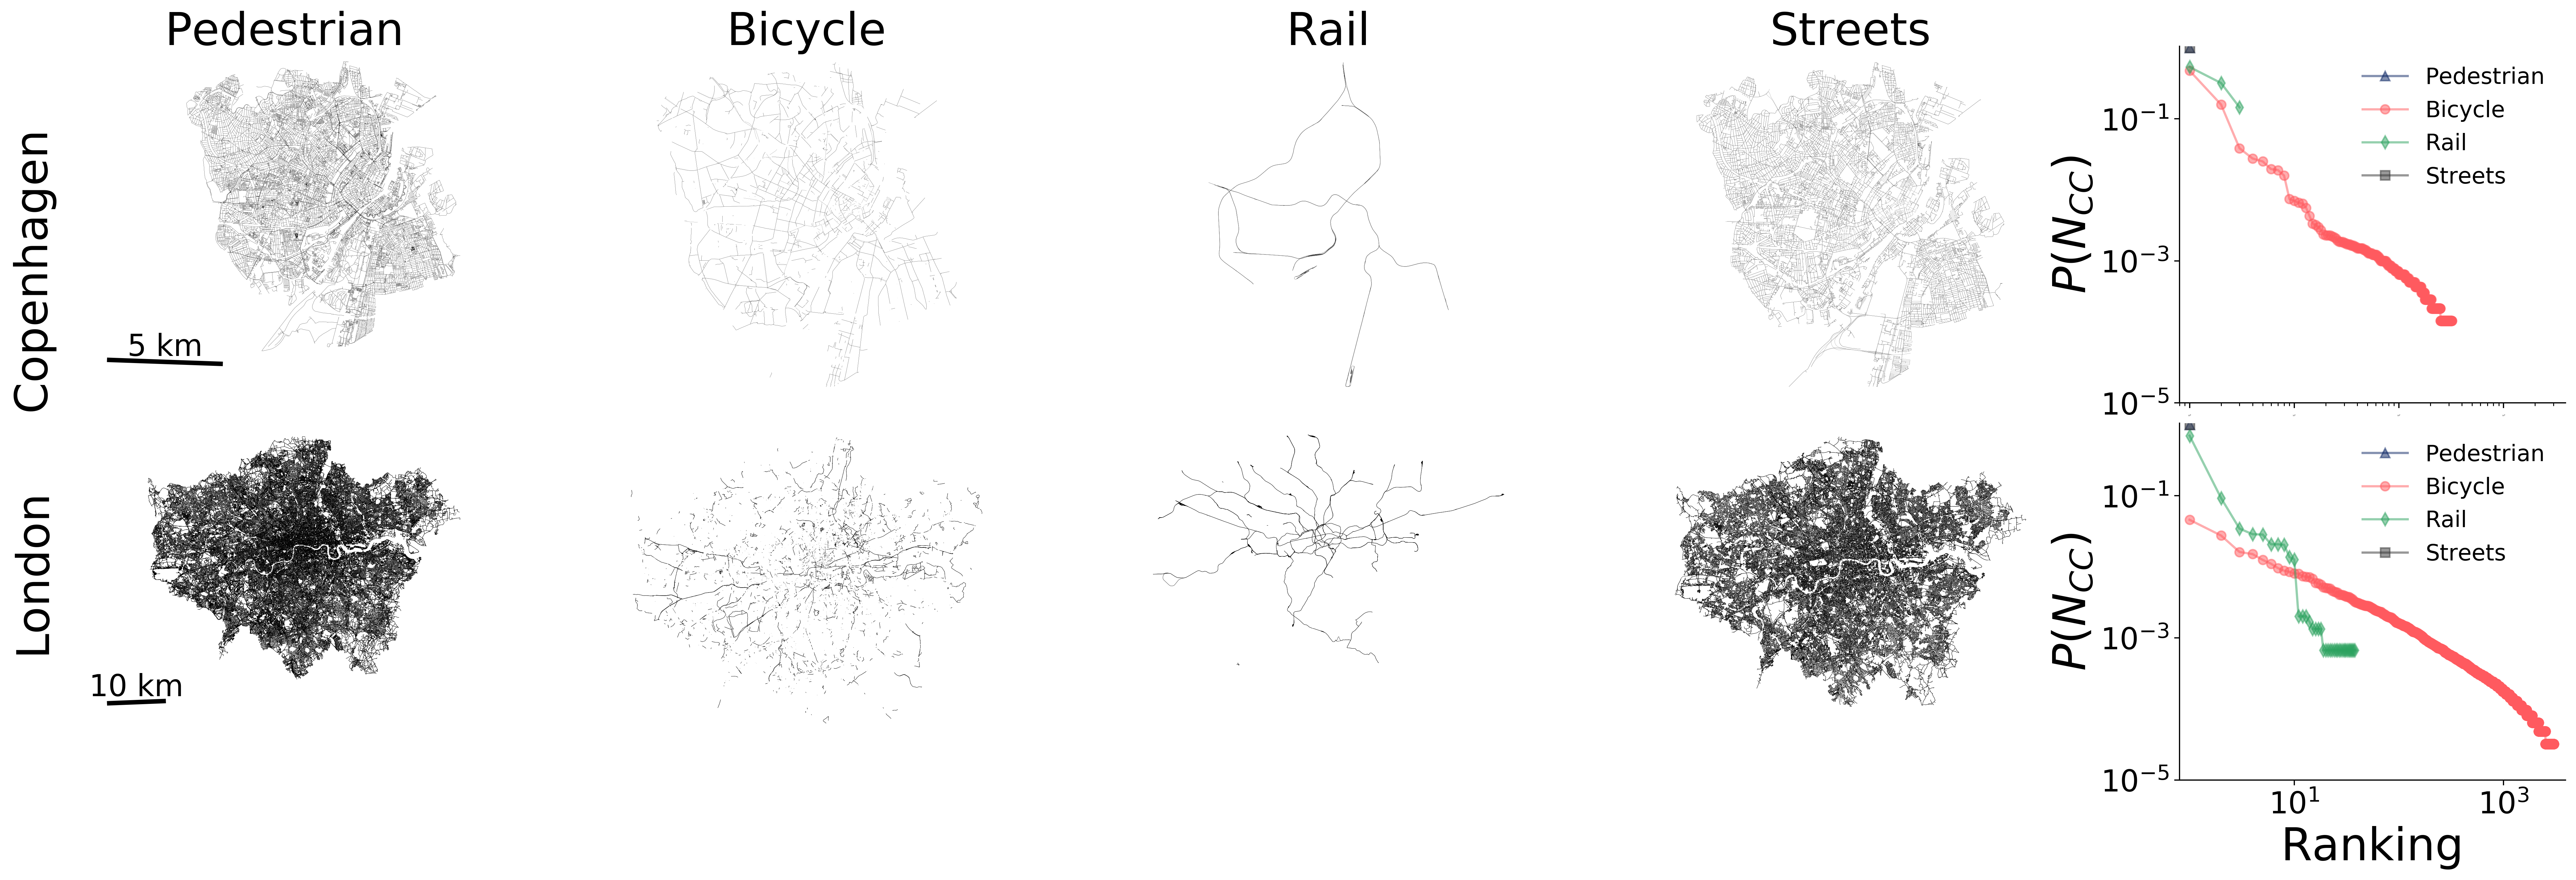
\includegraphics[width=\textwidth]{images/datadriven/Fig01.png}
  \caption[Multimodal configuration]{\textbf{(Map plots, left)} Networks representing various layers of transport infrastructure (pedestrian paths, bicycle paths, rail lines, and streets) for Copenhagen and London, with data from OpenStreetMap. \textbf{(Right)} Connected component size distribution $P(N_{cc})$ as a function of the ranking of the component for all considered network layers and cities. All layers are well connected except the bicycle layer: Copenhagen has 321 bicycle network components despite being known as a bicycle-friendly city, while London's bicycle layer is much more fragmented, featuring over 3000 disconnected components. Copenhagen's largest connected bicycle component (leftmost data point) spans 50\% of the network, but London's only less than 5\%.}
  \label{fig:Multimodal}
\end{figure}

\section{Data}
We acquired street and bicycle infrastructure networks from multiple cities around the world using OSMnx \cite{Boeing2017OSMNX}, a Python library to download and construct networks from OpenStreetMap (OSM). OSMnx simplifies the OpenStreetMap's raw data to retain only nodes at the intersections and dead ends of streets, and the spatial geometry of the edges, generating a length-weighted nonplanar directed graph \cite{Boeing2020Planarity}. These data sets are of high quality \cite{Haklay2010OpenStreetMap,Girres2010Quality} in terms of correspondence with municipal open data \cite{Ferster2019Bicycle} and completeness: More than $80\%$ of the world is covered by OSM \cite{Barbosa-Filho2017Models}. In particular, OSM's bicycle layer has better coverage than proprietary alternatives like Google Maps \cite{Hochmair2012}. We collect data from a diverse set of cities to capture different development states of bicycle infrastructure networks; from consolidated networks like Amsterdam and Copenhagen, less developed ones like Manhattan and Mexico City, to rapidly developing cities like Jakarta and Singapore. The various analyzed urban areas and their properties (number of nodes $N$, number of connected components $CC$, and population) are reported in Table~\ref{tab:DataDrivenCities}. Code to replicate our results is available as Jupyter Notebooks (\url{https://github.com/nateraluis/bicycle-network-growth}) and data can be downloaded from Harvard Dataverse \cite{natera2019data}.

\begin{table*}[th!]
  \centering
  \begin{adjustbox}{width=\textwidth,keepaspectratio}
    \begin{tabular}{llllllllllllll}
      \toprule
      {}         & \multicolumn{3}{l}{walk} & \multicolumn{3}{l}{bike} & \multicolumn{3}{l}{rail} & \multicolumn{3}{l}{drive} & Population                                                                                                             \\
      {}         & $N$                      & $CC$                     & $\ell(km)$               & $N$                       & $CC$       & $\ell(km)$ & $N$     & $CC$ & $\ell(km)$ & $N$       & $CC$ & \multicolumn{2}{l}{$\ell(km)$}              \\
      \midrule
      Amsterdam  & 23,321.0                 & 1.0                      & 2,075.67                 & 34,529.0                  & 355.0      & 972.08     & 1,096.0 & 8.0  & 288.72     & 15,125.0  & 1.0  & 2,010.49                       & 872,680    \\
      Barcelona  & 20,203.0                 & 1.0                      & 2,122.6                  & 7,553.0                   & 122.0      & 229.19     & 263.0   & 29.0 & 105.98     & 10,393.0  & 1.0  & 1,551.44                       & 1,600,000  \\
      Bogota     & 81,814.0                 & 1.0                      & 8,686.51                 & 9,760.0                   & 171.0      & 367.33     & 166.0   & 12.0 & 20.2       & 62,017.0  & 1.0  & 7,383.69                       & 7,412,566  \\
      Budapest   & 73,172.0                 & 1.0                      & 7,746.12                 & 10,494.0                  & 257.0      & 336.13     & 1,588.0 & 20.0 & 522.06     & 37,012.0  & 1.0  & 5,332.97                       & 1,752,286  \\
      Copenhagen & 30,746.0                 & 1.0                      & 2,286.66                 & 13,980.0                  & 321.0      & 417.01     & 276.0   & 3.0  & 123.56     & 15,822.0  & 1.0  & 1,547.3                        & 2,557,737  \\
      Detroit    & 47,828.0                 & 1.0                      & 6,769.46                 & 3,663.0                   & 53.0       & 141.06     & 20.0    & 3.0  & 11.54      & 28,462.0  & 1.0  & 5,624.49                       & 672,662    \\
      Jakarta    & 140,042.0                & 1.0                      & 13,947.96                & 248.0                     & 19.0       & 8.44       & 60.0    & 8.0  & 81.24      & 138,388.0 & 1.0  & 14,194.2                       & 10,075,310 \\
      LA         & 89,543.0                 & 1.0                      & 14,329.92                & 14,577.0                  & 230.0      & 653.16     & 173.0   & 9.0  & 90.82      & 71,091.0  & 1.0  & 13,324.46                      & 3,792,621  \\
      London     & 270,659.0                & 1.0                      & 23,846.62                & 62,398.0                  & 3,023.0    & 1,281.71   & 2,988.0 & 38.0 & 1,045.39   & 179,782.0 & 1.0  & 18,154.52                      & 8,908,081  \\
      Manhattan  & 13,326.0                 & 1.0                      & 1,320.78                 & 3,871.0                   & 105.0      & 111.42     & 349.0   & 5.0  & 197.51     & 5,671.0   & 1.0  & 1,022.13                       & 1,628,701  \\
      Mexico     & 108,033.0                & 1.0                      & 14,547.18                & 5,218.0                   & 52.0       & 332.37     & 371.0   & 18.0 & 253.48     & 95,375.0  & 1.0  & 13,732.39                      & 8,918,653  \\
      Phoenix    & 111,363.0                & 1.0                      & 14,314.0                 & 35,631.0                  & 141.0      & 1,221.18   & 105.0   & 4.0  & 71.64      & 73,688.0  & 1.0  & 11,841.49                      & 1,445,632  \\
      Portland   & 50,878.0                 & 1.0                      & 5,324.78                 & 24,252.0                  & 198.0      & 596.36     & 230.0   & 2.0  & 132.36     & 35,025.0  & 1.0  & 4,583.47                       & 583,776    \\
      Singapore  & 82,808.0                 & 1.0                      & 8,633.13                 & 12,981.0                  & 104.0      & 339.39     & 683.0   & 14.0 & 428.66     & 50,403.0  & 1.0  & 6,635.37                       & 5,638,700  \\
      \bottomrule
    \end{tabular}
  \end{adjustbox}
  \caption[Measures for analyzed cities]{Measures for the administrative area of analyzed cities. The number of connected components ($CC$) and nodes ($N$) for each layer in all cities of our dataset are highly diverse due to the varying developmental levels and focus of transport.
    \label{tab:DataDrivenCities}}
\end{table*}

We characterize each city street and bicycle infrastructure as a primal network, \cite{Porta2006Primal} in which nodes are intersections, while links represent bicycle paths, and designated bicycle infrastructure. This recent approach has been useful to demonstrate how cities grow \cite{Strano2012Evolution,Barthelemy2013Evolution}, how efficient \cite{Gallotti2014Efficiency} and dense they are, and to capture the tendency of travel routes to gravitate towards city centers \cite{Lee2017Morphology}. This network is described by an adjacency matrix $A=\{a_{ij}^{[\alpha]}\}$ where $a_{ij}=1$ if there is a link between nodes $i$ and $j$ and 0 otherwise.

\section{Defining bicycle network growth strategies and quality metrics}
Across all cities considered, we find that almost all network layers are made up of one giant component, except for the bicycle layer which is always fragmented into many disconnected components (see Table~\ref{tab:DataDrivenCities}). This discovery is remarkable given that the fragmentation occurs also in bicycle-friendly cities like Copenhagen (Fig.~\ref{fig:Multimodal}), showing that cycling infrastructure can be suboptimal even in the leading cycling cities on the planet. To quantify such an underdevelopment in the sustainable mobility infrastructure of cycling, we focus on the single layer of bicycle networks and on two well-established metrics in bicycle infrastructure quality assessment \cite{Krizek2005Discontinuities,movement2013Cycling,Dobrovolny2014Pedestrian,Twaddell2018Multimodal,Beck2019Space}: \textit{connectedness} and \textit{directness}. Connectedness indicates ``the ease with which people can travel across the transportation system'' \cite{Twaddell2018Multimodal}, and it is related to answering the question ``can I go where I want to, safely?''. Directness addresses the question ``how far out of their way do users have to travel to find a facility they can or want to use?'', and can be measured by how easy it is to go from one point to another in a city using bicycle infrastructure versus other mobility options, like car travel.

As our main approach, we choose to measure connectedness and directness over the designated bicycle infrastructure only, without considering travel on streets. Although it is possible to cycle on streets, growing evidence from bicycle infrastructure and safety research is unveiling serious safety issues for cycling when mixed with vehicular traffic \cite{Reynolds2009impact,Teschke2012route,Pucher2016Safer}. However, we also tested our algorithms on a combination of bicycle infrastructure plus streets for which the maximum speed is $30\,\mathrm{km/h}$, following common best-practice reasoning that low speed limits can make streets safe for cycling \cite{global2016global}. The results of these additional simulations are available in the Supplementary Information; they do not differ significantly from the case of designated bicycle infrastructure presented below, as the developed algorithms follow the same rules to connect the multiple components in both cases of segregated bicycle infrastructure only and of included bikeable streets.

To quantify connectedness, we first measure the number of disconnected components of each city's bicycle network. It is no surprise that car-centric cities have a highly fragmented bicycle infrastructure: for example, London has more than 3,000 disconnected bicycle infrastructure segments. However, even bicycle-friendly cities like Copenhagen have over 300 disconnected bicycle path components -- see the connected component size distribution $P( N_{cc} )$ in Fig.~\ref{fig:Multimodal}. This infrastructure fragmentation in the bicycle layer poses a challenge for a city's multimodal mobility options \cite{natera2020multimodal} and for the safety of its cycling citizens \cite{Dill2009infrastructure,Chataway2014Safety}.

\subsection{Algorithmic approach}

There are various approaches in developing automated strategies for bicycle infrastructure planning. Hyodo et al.~\cite{Hyodo2000Modeling} have proposed a bicycle route choice model to plan bicycle lanes taking into account facility characteristics. Other studies have used input data from bicycle share systems \cite{Bao2017Planning} or origin destination matrices \cite{Mauttone2017Design} to plan bicycle lanes. More recently, taxi trips have been used to identify susceptible clusters for bicycle infrastructure \cite{Akbarzadeh2018Design}. Here we attempt an alternative approach: Since hundreds of bicycle network components already exist in most cities, we aim at consolidating the existing infrastructure by making strategic connections between components rather than starting from scratch.


\begin{algorithm}[h!]
  \begin{algorithmic}[1]
    \Procedure{\textit{L2S}}{}
    \State $\textit{G} \gets \text{ bicycle network graph}$
    \State $\textit{wcc} \gets \text{ components of network G}$
    \For {i in length(wcc)-1}
    \State  \text{sort \textit{wcc} by components size}
    \State $\textit{cc} \gets \text{ two biggest components from \textit{wcc}}$
    \State $\textit{i\_j} \gets \text{ closest nodes between } cc_0 \text{ and } cc_1$
    \State $\text{connect } cc_0 \text{ and } cc_1 \text{ in } i\_j$
    \EndFor
    \EndProcedure
  \end{algorithmic}
  \caption{Largest-to-Second. \textcolor{blue}{The algorithm takes the bicycle network \textit{G} and a list of its weakly connected components \textit{wcc}, then it iterates over the weakly connected components, sorts them by their size (number of nodes inside each component), locates the closest pairs of nodes between the first and the second components. The process is repeated until all the components have been connected.}}\label{al:L2S}
\end{algorithm}

\begin{algorithm}[h!]
  \caption{Largest-to-Closest. \textcolor{blue}{The algorithm takes the bicycle network \textit{G} and a list of its weakly connected components \textit{wcc}, then it iterates over the weakly connected components, sorts them by their size (number of nodes inside each component), locates the largest connected component and the closest of the remaining components, the components are connected. The process is repeated until all the components have been connected.}}\label{al:L2C}
  \begin{algorithmic}[1]
    \Procedure{\textit{L2C}}{}
    \State $\textit{G} \gets \text{ bicycle network graph}$
    \State $\textit{wcc} \gets \text{ components of network G}$
    \For {i in length(wcc)-1}
    \State  \text{sort \textit{wcc} by components size}
    \State $cc_0 \gets \text{ biggest component from \textit{wcc}}$
    \State $cc_n \gets \text{ clossest component to } cc_0$
    \State $\textit{i\_j} \gets \text{ closest nodes between } cc_0 \text{ and } cc_n$
    \State $\text{connect } cc_0 \text{ and } cc_n \text{ in } i\_j$
    \EndFor
    \EndProcedure
  \end{algorithmic}
\end{algorithm}

Our approach takes into account the currently available bicycle infrastructure and uses an algorithmic process to improve the network by finding the most important missing links step by step. This way we focus on optimizing the connectedness metric, growing the bicycle infrastructure by making it more connected, merging parts into fewer and fewer components. We develop two iterative greedy algorithms that we check against a random and a minimum investment approach. The first algorithm, \emph{Largest-to-Second} (L2S), identifies in each step the largest connected component in the bicycle infrastructure network and connects it to the second largest (see algorithm~\ref{al:L2S} for details). The second algorithm, \emph{Largest-to-Closest} (L2C), also identifies the largest connected component, but connects it to the closest of the remaining bicycle infrastructure components (see algorithm~\ref{al:L2C} for details). In both algorithms, components are connected through a direct link between their two closest nodes. We use this technique as an approximation to the underlying street-shortest path -- since the most relevant shortest 100 connections typically range from $14$ to $500$ meters, roughly the length of two blocks, this approximation is reasonable. The algorithms repeat this process until there are no more disconnected components in the network.

To have a random baseline, we compare our algorithms with a \emph{Random-to-Closest} (R2C) component approach. In each step of this baseline approach, one component is picked at random and connected with the closest remaining one (see algorithm~\ref{al:R2C} for details). This baseline allows us to model a scenario where infrastructure is developed following a systematic but random linking approach -- in urban development this corresponds to uncoordinated local planning that randomly connects close pieces of bicycle infrastructure. We also implement a second baseline, the extreme case of \emph{Closest-Components} (CC), which prioritizes connecting the closest two components disregarding their size (see algorithm~\ref{al:CC} for details). This CC approach is equivalent to an ``invest as little as possible'' development strategy -- it builds up a minimum-spanning-tree-like structure  following a modified Kruskal's algorithm \cite{Kruskal1956Spanning}. All four algorithms connect components optimizing a well-defined criterion, finding the critical missing links in the network, and adding one new link per iteration. See Fig.~\ref{fig:algorithms} for a schematic of the four algorithms.


\begin{algorithm}[h!]
  \caption{Random-to-Closest. \textcolor{blue}{The algorithm takes the bicycle network \textit{G} and a list of its weakly connected components \textit{wcc}, then it iterates over the weakly connected components, randomly picks a component and connects it to the closest of the remaining components. The process is repeated until all the components have been connected.}}\label{al:R2C}
  \begin{algorithmic}[1]
    \Procedure{\textit{R2C}}{}
    \State $\textit{G} \gets \text{ bicycle network graph}$
    \State $\textit{wcc} \gets \text{ components of network G}$
    \For {i in length(wcc)-1}
    \State $cc_{ran} \gets \text{ random component from \textit{wcc}}$
    \State $cc_n \gets \text{ clossest component to } cc_{ran}$
    \State $\textit{i\_j} \gets \text{ closest nodes between } cc_{ran} \text{ and } cc_n$
    \State $\text{connect } cc_{ran} \text{ and } cc_n \text{ in } i\_j$
    \EndFor
    \EndProcedure
  \end{algorithmic}
\end{algorithm}

\begin{algorithm}[h!]
  \caption{Closest-Components. \textcolor{blue}{The algorithm takes the bicycle network \textit{G} and a list of its weakly connected components \textit{wcc}, then it iterates over the weakly connected components, calculate the distance between available components and connect the two closests ones. The process is repeated until all the components have been connected.}}\label{al:CC}
  \begin{algorithmic}[1]
    \Procedure{\textit{CC}}{}
    \State $\textit{G} \gets \text{ bicycle network graph}$
    \State $\textit{wcc} \gets \text{ components of network G}$
    \For {i in length(wcc)-1}
    \State $\Delta_{min} \gets \text{ clossest components in \textit{wcc}}$
    \State $cc_{0} \gets \text{ first component for }\Delta_{min}$
    \State $cc_{1} \gets \text{ second component for } \Delta_{min}$
    \State $\textit{i\_j} \gets \text{ closest nodes between } cc_{0} \text{ and } cc_{1}$
    \State $\text{connect } cc_{0} \text{ and } cc_{1} \text{ in } i\_j$
    \EndFor
    \EndProcedure
  \end{algorithmic}
\end{algorithm}

We apply the algorithms to the bicycle infrastructure inside the political demarcation of the cities, however it is possible to extend the methods and include bicycle highways and cross-city trails, since they use as input a set of spatial network components to connect. We opt to not include cross-city links, since they are a special case only available in a few regions and where adequate intra-urban bicycle infrastructure has already been established \cite{Hildebrandt2013BicycleHighways,Taciuk2018Bicycle}.

\subsection{Evaluating the algorithms impact}

To test how much cities improve their bicycle layers using these four algorithms, we define two metrics on the bicycle layer that operationalize the notion of connectedness: i) $n_{LCC} = \frac{N_{LCC}}{N} $, the fraction of nodes from the bicycle infrastructure inside the largest connected component ($N_{LCC}$) compared to the total number of nodes from the same type of infrastructure ($N$), and ii) $\ell_{LCC} = \frac{L_{LCC}}{L} $, the fraction of link kilometers inside the bicycle infrastructure largest connected component ($L_{LCC}$) compared to the total number of link kilometers in the bicycle network ($L$). Both metrics take values between 0 and 1, where 1 means that there is only one connected component. An intermediate value, for example 0.2, means that the largest connected component contains 20\% of all bicycle intersections or path kilometers. Executing our algorithms step by step these metrics can only grow, approaching 1 when the process is complete and they terminate. What distinguishes the algorithms is \emph{how fast} these values grow.

\begin{figure}[t!]
  \centering
  \includegraphics[width=\textwidth]{images/datadriven/algorithms.png}
  \caption[Algorithms schematic representation]{Schematic representation of algorithms to improve bicycle network infrastructure: Largest-to-Closest (L2C) finds the largest component and connects it with the closest one; Largest-to-Second (L2S) connects the largest component with the second largest; Closest-Connected (CC) connects the two closest components; and Random-to-Closest (R2C) picks a random component and connects it to the closest.}
  \label{fig:algorithms}
\end{figure}

We quantify directness through the metric: iii) bicycle-car directness $\Delta$, which answers the question ``how direct are the average routes of bicycles compared to cars?'' via the ratio between average distance by car and average distance by bicycle. For example, if the shortest car-route from west to east Manhattan is 4\,km and the shortest route on the bicycle network between these two points is 5\,km, the bicycle-car directness is $4/5 = 0.8$. Note that if the bicycle network is a subset of the street network, then $\Delta$ cannot be larger than $1$. Formally we write $\Delta=\frac{\langle\delta_{ij}^b\rangle_{ij}}{\langle\delta_{ij}^s\rangle_{ij}}$, where $\langle\delta_{ij}^{s}\rangle_{ij}$ is the average car-route distance, and $\langle\delta_{ij}^{b}\rangle_{ij}$ is the average length of the shortest bike-route between $i$ and $j$. In each iteration of any of our algorithms, we implement this measure by randomly selecting one thousand pairs of origin-destinations nodes and then averaging the corresponding street/bicycle distance. To avoid undefined values due to disconnected components in the bicycle layer, we add the following condition: If a node from the pair \textit{i} and \textit{j} is in a different component, we assign the value $\delta_{ij}^{b} = 0$. This condition also ensures consistency of growing directness values while the algorithm merges more and more nodes into the same component.

Finally, in order to measure the cumulative efficiency of our algorithms, we define the metric: iv) $G_{LCC}$ as the relative gain of bicycle path kilometers in the largest connected component. For example, $G_{LCC}=1.5$ means that the algorithm has increased the largest connected component's original size by 150\%. Formally, $G_{LCC}=\frac{L_{LCC}-L_{LCC_0}}{L_{LCC_0}}$, where $L_{LCC_0}$ is the sum of kilometers in the largest connected component before the algorithm runs. As with all other metrics, $G_{LCC}$ is monotonically increasing with the growth algorithm, and reaches $\frac{1-\ell_{LCC_0}}{\ell_{LCC_0}}$ at the end of the dynamics.

\section{Growing bicycle networks shows stark improvements with small investments}

\begin{figure}[th!]
  \centering
  \includegraphics[width=\textwidth]{images/datadriven/BPincrease.png}
  \caption[Algorithmic improvement in Budapest]{\textbf{(a)} Normalized increase in nodes inside the largest connected component ($n_{LCC}$). \textbf{(b)} Normalized increase in kilometers inside the largest connected component ($\ell_{LCC}$). \textbf{(c)} Kilometers gain ($G_{LCC}$). \textbf{(d)} Bicycle-car directness ($\Delta$). Measures in (b-e) are plotted as a function of the sum of added links in kilometers, for the case of Budapest (for all cities see Fig.~\ref{fig:Nodes})}
  \label{fig:ImprovementBP}
\end{figure}

We demonstrate in Fig.~\ref{fig:ImprovementBP} the power of the various growth strategies by showing the initial state of the bicycle layer for the case of Budapest and its state after 85 iterations of the \emph{Largest-to-Closest} algorithm: At this point the network has almost quadrupled the size of its largest connected component (from 82\,km to 313\,km), with a negligible investment of just less than 5\,km (corresponding to $1.4\%$ of the previously existing bicycle infrastructure) in new connecting bicycle paths. In terms of connectedness, it goes from $15\%$ to $56\%$ connected. This rapid increase shows that the city can easily improve its bicycle infrastructure with small investments. For some extreme cases, like Bogota, with the same 5\,km investment (an increase of $1.3\%$ to the previously existing infrastructure) the bicycle-car directness increases from $6\%$ to almost $48\%$ and connectedness from $34\%$ to $89\%$. \textcolor{blue}{Similar encouraging results hold for other cities (See Section~\ref{SI:BikeImprovement}).}%, and for all the cities when taking into account the combination of bicycle infrastructure and safely bikeable streets ($\leq 30\,\mathrm{km/h}$), in Figure~\ref{fig:Lengthsncrease_BikeStreets} we show the increase in bikable kilometers when taking into consideration the  (see SI).

The fraction of nodes inside the largest connected component increases rapidly with newly added links for all considered algorithms except \emph{Random-to-Closest}, Fig.~\ref{fig:ImprovementBP}(a). The \emph{Largest-to-Closest} algorithm performs better than the others, even more than \emph{Closest-Components} which prioritizes minimum investments in the network. Since we are considering bicycle infrastructure, a better practical measure than the number of intersections is the number of kilometers that can be cycled using only designated paths. Figure~\ref{fig:ImprovementBP}(b) shows how this measure improves in a similarly explosive way: with an investment of only 20\,km ($5.9\%$ of the existing infrastructure), the largest connected component will contain $~80\%$ of the original bicycle infrastructure. Results for the kilometer gain $G_{LCC}$ are shown in Fig.~\ref{fig:ImprovementBP}(c). Three of the four algorithms rapidly gain new kilometers, but as the invested new kilometers grow, each algorithm follows a different gain rate. Also for this metric, \textit{Largest-to-Closest} is the algorithm with the best performance.

\begin{figure*}[ht!]
  \centering
  \includegraphics[width=0.8\textwidth]{images/datadriven/SI_Lengths_Bike_Streets.png}
  \caption{Normalized increase in kilometers inside the largest connected component ($\ell_{LCC}$).}
  \label{fig:Lengthsncrease_BikeStreets}
\end{figure*}

We also measure the bicycle-car directness ratio, Fig.~\ref{fig:ImprovementBP}(d). The bicycle-car directness $\Delta$ improves as the algorithms consolidate the network. These improvements are, however, indirectly driven by the improvement of connectedness, which boosts the accessibility of bicycles to different areas of the city. The flattening of the curves at a value considerably smaller than 1 (around 0.65) shows that cars will always outperform bicycles in terms of directness, having on average at least 33\% shorter paths in the city. This suboptimal flattening is a natural consequence of the algorithms optimizing for connectedness only, not adding ``redundant'' connections. Nevertheless, the measure shows that, similar to connectedness, with a relatively negligible investment of bicycle path kilometers into the system, the bicycle network's directness improves drastically, even in the greediest case where the shortest possible missing link is added in every iteration. This result holds for all analyzed cities (see SI). The large differences between the baseline \emph{Random-to-Closest} and our two algorithms (\emph{Largest-to-Second} and \emph{Largest-to-Closest}) show the importance of following an approach that consolidates and grows the largest connected component. \textcolor{blue}{Similar results are obtained for all the cities when taking into account the combination of bicycle infrastructure and safely bikeable streets ($\leq 30\,\mathrm{km/h}$), in Figure~\ref{fig:Lengthsncrease_BikeStreets} we show the increase in bikable kilometers when taking into consideration bikable streets and designated bicycle infrastructure combination for all the analyzed cities (see Section~\ref{SI:BikeStreets} for the rest of the measures).}

\section{Different cities have different optimal investment strategies}

\begin{figure}[htp!]
  \centering
  \includegraphics[width=\textwidth]{images/datadriven/5km.png}
  \caption[Cities bicycle connectivity improvement 5 new kilometers]{Cities improvement and ranking using the \emph{Largest-to-Closest} algorithm. We report the improvement and ranking on the fraction of total kilometers of bicycle infrastructure in the largest connected component ($\ell_{LCC}$) and in the bicycle-car directness ($\Delta$). Dotted lines show thresholds of $25\%$, $50\%$, and $75\%$. Plots (a-b) show investment strategies of 5\,km and 35\,km, respectively, the Manhattan, London, and Budapest plots show the suggested new links (red) after adding 5\,km and 35\,km, the newly created largest connected component (black), and the remaining separated components (grey).}
  \label{fig:Improvement5}
\end{figure}

Differences arise in the state of the bicycle layer and its improvement after applying a growth algorithm. To see this effect, we rank how cities improve using the \textit{Largest-to-Closest} algorithm in two different investment scenarios: investing either i) 5\,km, or ii) 35\,km. Figure~\ref{fig:Improvement5} shows how cities improve when investing 5\,km of bicycle infrastructure. We see that some cities get above $75\%$ of their existing infrastructure connected, meaning that their bicycle layer only needs a small extension. On the other hand, cities like London, Los Angeles, and Jakarta need a larger investment to improve. Concerning bicycle-car directness, cities reach lower values due to the focus of the algorithms on completeness. In the worst performing cities like Los Angeles, a covered length close to $50\%$ can be reached easily, while the bicycle-car directness ratio stays below $20\%$, showing that it is much harder to gain an acceptable bicycle infrastructure in cities where cars are overprioritized. The 35\,km investment strategy shows that most cities can get at least $75\%$ of their bicycle infrastructure connected, Fig.~\ref{fig:Improvement35}. The worst performing outlier is London, due to its bicycle layer containing more than 3000 connected components scattered around $1600$ km$^2$ (see Table \ref{tab:DataDrivenCities}). In terms of bicycle-car directness London also performs badly, while Amsterdam is the best performing one.

\begin{figure}[htp!]
  \centering
  \includegraphics[width=\textwidth]{images/datadriven/35km.png}
  \caption[Cities bicycle connectivity improvement 35 new kilometers]{Cities improvement and ranking using the \emph{Largest-to-Closest} algorithm. We report the improvement and ranking on the fraction of total kilometers of bicycle infrastructure in the largest connected component ($\ell_{LCC}$) and in the bicycle-car directness ($\Delta$). Dotted lines show thresholds of $25\%$, $50\%$, and $75\%$. Plots (a-b) show investment strategies of 5\,km and 35\,km, respectively, the Manhattan, London, and Budapest plots show the suggested new links (red) after adding 5\,km and 35\,km, the newly created largest connected component (black), and the remaining separated components (grey).}
  \label{fig:Improvement35}
\end{figure}

The four proposed metrics capture the impact of newly created connections on the various components of the bicycle network. By linking previously disconnected neighbourhoods with a sustainable mode of transport, our approach focuses on consolidating bicycle infrastructure networks, thus making cities more cohesive and green. It does not, however, focus on growing the bicycle network into large areas of the city not currently served. To test to which extent such connectedness-based algorithms bring an indirect benefit for coverage, we measured the proportion of the city that is covered and reachable by bicycle with an epsilon of 500 meters around the bicycle infrastructure of the largest connected component, and calculated the percentage of nodes in the street layer that are covered by the bikeable area. The results of this measurement show a wide range of effects: Cities with an already high coverage above 80\% (Amsterdam, Copenhagen) reach near instantly 100\%, cities with an intermediate coverage (Manhattan, Bogota, Budapest) follow a more linear progression per added kilometer, while underdeveloped or sprawling cities (LA, London, Jakarta) show negligible growth (Fig.~\ref{fig:Coverage}).

\begin{figure*}[th!]
  \centering
  \includegraphics[width=0.8\textwidth]{images/datadriven/Reviewer_Coverage.png}
  \caption[Bicycle infrastructure service area]{Area of influence (coverage) for the bicycle infrastructure in the street layer.}
  \label{fig:Coverage}
\end{figure*}

While our present goal (consolidation of the bike network) is intended to show the potential of our approach, an extension towards the exploration of new city areas will increase further the real-world applicability of our results. We consider this extension an interesting line of future research in the challenge of developing optimal data-driven strategies of transport network growth, potentially informed by theoretical frameworks such as optimal percolation~\cite{achlioptas2009explosive,morone2015influence}. Besides, the use of other network metrics, such as network efficiency~\cite{latora2000efficient}, might unveil new dimensions characterising the impact of the proposed algorithms on the development of the bicycle infrastructure.


\section{Discussion}
Our starting point showed that a common characteristic of cities is the fragmentation of their bicycle networks. We have proposed the use of data-driven algorithms to consolidate bicycle network components into connected networks to improve efficiently sustainable transport. We have shown that connecting the bicycle infrastructure in an algorithmic way rapidly improves the connectedness and directness of the bicycle layer. These algorithms, when compared with two baselines, highlight the usefulness of growing the bicycle network on a city-wide scale (considering all areas of the city) rather than randomly adding local bicycle infrastructure. Improving the connectivity of bicycle lanes and paths improves not only the network itself, but also promotes the use of bicycles as means of transportation in a city, improving the health of its inhabitants \cite{Mueller2018Health}.

Improving bicycle infrastructure one link at the time (by identifying suitable components to connect) is only the first step towards a systematic framework for realistic bicycle network growth strategies. Our current approach is not the last word in this development, since it does not yet explicitly optimize for directness and does not account for transport flow. Further, our proposed approach helps implement a more connected transport network which can improve the possibilities for multimodal transport. This could be starting point for implementing truly multimodal strategies, such as integration with public transportation, or bicycle parkings in transportation hubs \cite{Twaddell2018Multimodal}.

In our algorithms, each new link works as a bridge between components, potentially having large betweenness centrality. Such high-betweenness segments could become overused and create bottlenecks in practice. To improve this situation, it would be necessary to create links in the network that act as redundant paths. In doing so, directness and coverage would also be improved, along with the network's robustness to interruptions. This is an interesting and possibly demanding task that we leave for future research, as the new links would have to be created in a coherent manner balancing trade-offs between network structure and mobility dynamics. We anticipate that complementing OpenStreetMap data with additional information on the use of traffic flow and movement data, like trips from bike share systems or origin-destination matrices, possibly from alternative sources such as municipalities and transportation agencies, might further improve the algorithms by better detecting underserved and optimal areas in the city where new links should be created. Despite these various possibilities for qualitative updates to the studied growth strategies, our first models have demonstrated the capability to generate substantial improvements with minimal effort.

The use of data-driven algorithms to identify crucially missing links in bicycle infrastructure has the potential to improve the mobility infrastructure of cities efficiently and economically. This approach is not only useful for planning city structure, but could also be used together with simulating mobility flows and to provide insights on how the system will behave after new measures are implemented. Ultimately, planning cultures and processes will also have to be accounted for \cite{zhao2018bicycle}. We anticipate that a future stream of work should include longitudinal studies \cite{carstensen2015spatio} in multiple cities, along with algorithmic simulations to first model and simulate possible changes to the transport network, and then to test those models with ground truth data, to compare the evolution of infrastructure and mobility dynamics between cities with different transport priorities.\pagestyle{fancy} %Bike algorithms
\chapter{Life quality as walkability}\label{ch:LQI}

Life quality in cities is deeply related to the mobility options, and how easily one can access different services and attractions. The pedestrian infrastructure network provides the backbone for social life in cities. While there are many approaches to quantify life quality, most do not take specifically into account the walkability of the city, and rather offer a city-wide measure. Here we develop a data-driven, network-based method to quantify the liveability of a city. We introduce a life quality index (LQI) based on pedestrian accessibility to amenities and services, safety and environmental variables. Our computational approach outlines novel ways to measure life quality in a more granular scale, that can become valuable for urban planners, city officials and stakeholders. We apply data-driven methods to Budapest, but as having an emphasis on the online and easily available quantitative data, the methods can be generalized and applied to any city.\footnote{A stand alone version of this chapter has been published in Complex Networks and Their Applications VIII \cite{natera2020walkability}.}
\pagebreak

\section{Walking the city}
In this chapter, we shift our attention from the bicycle, to the pedestrian layer. We focus on measuring the livability of a city using its pedestrian infrastructure to compute how easy it is to access different types of amenities that serve multiple purposes, such as cultural, educational and access to day-to-day goods.

As mentioned in the previous chapters, the evolution that most cities followed during the 20th century promoted a car-centric vision~\cite{Jacobs1961Death,Gossling2016Space,Szell2018Crowdsourced}, neglecting the presence of other mobility options. From a liveability perspective, this situation is suboptimal because the automobile infrastructure dominates and defines the walkable area, increasing car traffic, air pollution and deteriorating walkable conditions.

The concept of walkability is an important factor to consider in connection with liveability. Liveability refers to an environment from an individual perspective~\cite{Heylen2006Liveability} which includes ``a vibrant, attractive and secure environment for people to live, work and play and encompasses good governance, a competitive economy, high quality of living and environment sustainability''~\cite{Shamsuddin2012Walkable}. Thus, in a liveable city, there must be an emphasis not only on sustainable transportation and built environment to reduce the harm on nature~\cite{Campbell1996Green,Jabareen2013Planning} but also encouraging citizens to walk for supporting their physical and mental well-being~\cite{Frank2006Many}. However, improving walkability is more complex than we would think. Walking should be an available, safe and well-connected mode of transportation, but as Speck put it well, it should be interesting and comfortable as well, to have a feeling of the streets as ’outdoor living rooms’~\cite{Speck2012Walkability}.

The pedestrian infrastructure that sustains walkability in a city can be described as a network~\cite{porta2006primal}. This approach has been useful to identify street patterns~\cite{barthelemy2008patterns,louf2014typology} and its evolution~\cite{strano2012evolution,Barthelemy2013Evolution}, measure the morphology of cities~\cite{Boeing2019Morphology}, and how the streets' connectivity impacts on pedestrian volume~\cite{Hajrasouliha2015Impact}.

The various approaches to create a walkability index or so-called walk score consider mainly the following components: safety and security~\cite{Quercia2015Digital,Silva2018Investigating}; convenience, attractiveness and public policy~\cite{Krambeck2006Global,Speck2012Walkability}, connectedness~\cite{Southworth2005Designing}, but also reckon with the land use mix and residential density of the certain area\cite{Carr2010Walk}. Another approximation rather accents the importance of its effect on air pollution, health problems, travel costs and even on the sense of community\cite{Stephen2014Sustainable}. Thus measuring walkability not only captures the propensity to walk in a city but also includes the components a liveable city must have and support, under the umbrella of sustainability.

There are good examples of how sustainable city development initiatives tackle growing inequalities with data-driven approaches. Long Island used city data to analyze which amenities are needed to increase the quality of life in a newly built environment~\cite{Childs2018Planning}, other cities are investing in smart technologies to develop public transport, connecting spatially discriminated areas~\cite{Kaushik2017Planning,Fitzgerald2016Data}.

Since the number of components which should be taken into consideration in creating a walkability index is high, the types of data are also mixed and thus difficult to integrate. While the information on connectedness, security, residential density, etc. is quantitative and in general easily available, gaining opinion about attractiveness, convenience, or even about the feeling of security is more complicated. Here we propose to use a data-driven approach as a proxy to quantify life quality, making it reproducible and easily expanded to include different data sources. We apply our methods to Budapest, but as having an emphasis on the online and easily available quantitative data, the methods can be generalized and applied to any city.

\section{Data: Pedestrian network, points of interest, and city attributes}
\subsection{Pedestrian network}
We work with three different data sources: networks, points of interest and city attributes. To acquire the pedestrian network and points of interest, we used OSMnx~\cite{boeing2017osmnx}, the same tool we used in the previous chapters (see Chapter~\ref{sec:datatools}). As we have shown, the data from open street maps is of high quality~\cite{haklay2010openstreetmap,girres2010quality,Ferster2019Bicycle}, and completeness~\cite{barbosa2018human}. The obtained network contains all the sidewalks and pedestrian designated infrastructure, it is conceptualized as undirected, nonplanar and primal network~\cite{porta2006primal}. This network is described as a weighted graph, with its adjacency matrix $W=w_{ij}$ where the weight $w_{ij}$ contains the length between $i$ and $j$ if connected, and $0$ otherwise. We also encoded in the links the traversal time $Tt_{ij}$ between nodes $i$ and $j$ calculated as $Tt_{ij}=\frac{\ell_{ij}}{ps}$ where $ps$ is the pedestrian speed as a constant rate of $5km/h$.

\subsection{Points of interest}
The majority of points of interest were downloaded from OpenStreetMap, from different classification keys (amenity, tourism, shop, office, leisure) using OSMnx~\cite{boeing2017osmnx}. We filtered the points of interest using the districts' demarcation~\cite{HU2019Districts}, to get only the data within Budapest boundaries, having, as a result, more than $39,000$ data points. We complement the data sets with secondary data sources as specialized directories of doctors and childcare facilities (see Section~\ref{SI:walkabilityData}).

We categorize the points of interest in six main categories: I) Family friendliness (Access to education and daycare, and family support services), II) Access to health care and sport facilities, III) Art and culture (e.g. museums, exhibitions), IV) Nightlife (e.g. bars, restaurants), V) Environment (air quality and access to green areas), and VI) Public Safety. The points of interest and secondary data sources are available at \url{https://github.com/nateraluis/Budapest_LQI}

\subsection{City attributes}
The district-level data (population and crimes) were obtained from the Hungarian Police's public database. The crime statistics are reported as the  number of crimes committed in public places in 2018~\cite{HU2019Police}. Population data is coming from the 2016 micro-census conducted by the Hungarian Statistical Bureau~\cite{HU2016Population}. We took into account the air pollution, this data set coming from National Air Pollution Measurement Network~\cite{HU2019Pollution}, containing the geolocation of the air quality stations and different measures (annual median concentration of carbon monoxide, nitrogen dioxide, and PM10 dust).

Accuracy of the Life Quality Index (LQI) model highly depends on how comprehensive the distribution of listed services. We use OSM as our key data source, but to achieve a more comprehensive and country-specific database we collect publicly available data from various Hungarian websites for each category. %(See Appendix A for databases and sources)

To project the city attributes to the network we assigned properties to its nodes. Matching them with their corresponding districts, then assign attributes to the nodes based on the district level data (population and crimes, see section \ref{safety}). For the pollution data, we calculated the corresponding Voronoi cells for the air quality stations, and matched the nodes with them. Finally, we divided the pollution by the number of nodes in each corresponding cell and assigned the value to the nodes (See section \ref{environment}). 

\begin{figure*}[ht!]
	\centering
	\includegraphics[width=\textwidth]{images/lqi/Budapest_Network_voronoi_op2.png}
	\caption[Budapest pedestrian network]{\textbf{(a)} Network representing Budapest pedestrian structure. The network was built following a primal approach, where the edges are sidewalks and pedestrian infrastructure, and nodes are intersections. \textbf{(b)} The graph-Voronoi tessellation of the Budapest network, generated using a subset of 15 parks as seeds. The color of the nodes represents the cell they belong to and the highlighted red dots are the seeds of each cell. The distance measure between two points is defined as the weighted shortest path on the graph, the weights being the average time required to cross a given edge.}
	\label{fig:BPnetwork}
\end{figure*}

\section{Quantifying life quality}
The life quality of a person is largely subjective and hard to quantify. However, it is both intuitive and has been scientifically shown that the environment and personal well-being strongly correlate~\cite{Rosow1961Social}. Thus using environmental factors as proxies, life quality and livability becomes quantifiable~\cite{Kahneman2006Developments}.

The main environmental factors we consider in our model are: the availability of services and amenities, the quality of the infrastructure, environmental factors and safety. The goal of our model is to quantitatively characterize the immediate environment of residents in the space of factors that affect life quality.

The fundamental framework of our model and our calculations is the network representation of Budapest’s pedestrian infrastructure. The nodes of the network represent intersections, while links are sidewalks and pedestrian infrastructure. The output of our model is an index, that characterizes every node of the Budapest network, giving a high-resolution quality-landscape of the city. The index is ultimately a number aggregated from multiple sub-categories, and its main value is highlighting inequalities and relative deficiencies within the city.

The final value of the index is a weighted sum, characterizing every node (intersection) in the network:
\begin{equation} \label{final_Q}
	Q_i =w^{services}\Tilde{Q}_i^{services} + w^{safety} \Tilde{Q}_i^{safety} + w^{environment}\Tilde{Q}_i^{environment}
\end{equation}
In the equation $i$ represents an individual node in the network. The ``tilde'' above the $Q$ terms means that the values of the different category indices are normalized within the category. The weights $w$ assigned to every term are arbitrary and are highly context-dependent. All terms of the equation are discussed in the following sections.
%We include the weights used for producing the results of this chapter in Appendix B.

The weights of the different $Q$ indices in the final aggregation highly depend on the context and the nature of the problem. For this study we followed a participatory design process~\cite{kunze2011conceptual,gaziulusoy2017shifting,heitlinger2018avoiding}, actively involving stakeholders to define them. This process let us incorporate practical knowledge of the importance of the services, safety and the environment in a city.

The weights of the sub-indices from equation (\ref{final_Q}) are of the following values:

\begin{itemize}
  \item $w^{\text{services}}=0.7$;
  \item $w^{\text{safety}}=0.1$;
  \item $w^{\text{environment}}=0.2$
\end{itemize}

\subsection{Services index}
The number quantifying each node in terms of how well it is connected with amenities and services is a weighted sum of sub-categories as well.
\begin{equation}\label{Q_services}
	Q_i^{services} =\sum_c w^c Q_i^c
\end{equation}

where, $c$ denotes categories (family, culture, health, sport, and nightlife), and $w^c$ the importance of category $c$. 

As when building the aggregated index, we also followed a participatory process to account for the importance of different category-services in the city. The weights used in equation (\ref{Q_services}) are as follows:

\begin{itemize}
  \item $w^{\text{family}}= 0.3$;
  \item $w^{\text{health}}= 0.3$;
  \item $w^{\text{culture}} = 0.15$;
  \item $w^{\text{sport}} = 0.15$;
  \item $w^{\text{night life}}=0.1$
\end{itemize}

Some categories, like family, have further subcategories. Even though we have also had data and made a separate analysis on tourism, its effects on life quality of the residents are ambiguous, so we decided to omit it from the index.

What sets categories apart is that they incorporate different sets of amenities, with a few overlaps. The details of the categorization of amenities are included in the Appendix.

For every service/amenity class we have a given set of points of interest (POI) along with where the amenities of that class are available, with exact geo-location. We assign every POI of a given amenity class (e.g. supermarket, pharmacy, school, etc.) to the nearest node on the infrastructure network. Each set of POIs organically generates a spatial partitioning of the city with one partition per POI. The partition of a POI is the set of all the nodes from which that particular POI can be reached faster than any other POI of the same class.

Mathematically these partitions are called graph-Voronoi cells~\cite{Erwig2000Graph,Deritei2014Community}, where every node of a cell is assigned to its closest seed (POI). Distance, in this case, is not euclidean or geometric distance, but the distance on the network, where we use the weighted shortest path between two nodes as the distance measure. The weight of links is a temporal parameter encoding the average time required to cross the represented street from one end to the other, thus the weight is a simple product of average speed and length of the street. This is in principle very similar to the way navigation systems find routes between points. For an example of a graph-Voronoi partitioning see Figure~\ref{fig:BPnetwork} (b).

To assess how well-connected a node is to amenities we consider the following factors:
\begin{itemize}
	\item How important is an amenity - weight ($w_a$)
	\item How long does it take to reach the amenity - time to reach ($t_ia$)
	\item Relatively how many nodes (or people) does the amenity share with - exclusivity ($P_a$)
\end{itemize}

From the three factors, the latter two are calculated using the city infrastructure network. The index for an amenity class, from the perspective of node $i$, is proportional with its importance (weight) and it is inversely proportional with the time to reach the closest POI from $i$ and with the degree of exclusivity.

\begin{equation}\label{q_i}
	q_i^a=\frac{w_{a}}{(P_a+1)(t_{ia}+1)}
\end{equation}

There can be certain singular cases when a Voronoi cell is empty ($P_a=0$, i.e. no residents in the area) or the node i in question is right at the POI ($t_{ia}=0$). To avoid anomalies in the index we added 1 to both parameters.

The index of one category is proportional to the sum of its amenity-indices (calculated in (\ref{q_i})). To treat this number on the right scale (in practice we can get very large and very small numbers) we take the natural logarithm of the sum across amenities.

\begin{equation}
	Q_i^c=log(\sum_a q_i^a):
\end{equation}

As we have mentioned earlier, the final services index is the weighted sum of the indices of the sub-categories.

$$Q_i^{services} =\sum_c w^cQ_i^c $$

Finally, we normalize the values of $Q^{services}$, so its values are comparable to the other values of the final $Q$ equation (\ref{final_Q}):
\begin{equation}
	\Tilde{Q}_i^{services} =\frac{Q_i^{services}+|min(Q^{services})|}{max(Q^{services})+|min(Q^{services})|}
\end{equation}

Even if there are potentially other ways to build a life quality index, this is a synthetic way of doing it that can be used as a tool for policymakers to evaluate the urban conditions and how they relate to the quality of life in a given city. In particular, this approach has been used in Budapest to evaluate the current urban conditions and to plan future developments. More recently, a variation of this approach was used to evaluate the impact of new cyclist infrastructure during the beginning of the COVID-19 pandemic in Budapest. \textcolor{red}{ The variation took into consideration the existing pedestrian and bicycle infrastructure. We built a network combining both infrastructures and measure the accesibility with the proposed method to stablish baseline. Then, we incorporated the pop-up temporary bicycle infrastructure into the previously built network and evaluate  how the accesibility changed. A set of preliminary results were presented to the Budapest municipal government for their consideration.}

\subsection{Safety index} \label{safety}

The safety index is calculated across districts based on the number of crimes committed per one hundred thousand residents. Since the highest resolution data available to us was on the district level, every node $i$ in the same district will have the same safety index value. The crime index:

$$Q_i^{crime}=\frac{N^{district}_{crime}}{n_i^{district}}$$
Where $N^{district}_{crime}$ is the number of crimes committed in a district in a year, and $n_i^{district}$ is the number of nodes in the district. The safety index is one minus the normalized crime index.
\begin{equation}
	\Tilde{Q}_i^{safety}=1-\frac{Q_i^{crime}}{max(Q^{crime})}
\end{equation}

\subsection{Environmental index} \label{environment}

The environmental index is made up of two components: air pollution ratio and ratio of natural areas.

\subsubsection{Air pollution ratio}
We use the data provided by Budapest’s air pollution measuring stations for the year 2018. For this study, we used the yearly median value of three polluters: carbon monoxide, nitrogen dioxide, and PM10 dust-pollution.
As an approximation, we project the geometric Voronoi cells of the measuring stations onto the city map and each node will receive the pollution metrics of the geometrically closest station. We divide these values with the yearly upper health limit for the given polluter to assess to what degree do these values approximate the health limit. Thus the air pollution index of one node is formalized as follows:
$$C_i=\frac{c_i^{CO}}{c_{limit}^{CO}}+\frac{c_i^{NO_2}}{c_{limit}^{NO_2}}+\frac{c_i^{Pm10}}{c_{limit}^{Pm10}}$$

Where $c^{CO}_{limit}=3000 g/m^3$, $c^{NO_2}_{limit}=40 g/m^3$ , $c^{Pm10}_{limit}=40 g/m3$ are the yearly upper limits based on data from the Hungarian Air Quality Network~\cite{HU2019Pollution}.

\subsubsection{Ratio of natural areas}
For this index, we have data on the neighborhood level, which is a more granular level of administrative partitioning the city than the districts are. In this case, we project the same index onto every node in the same neighborhood. We consider as natural areas forests, parks and water surfaces (ponds, rivers, etc). \\
The index:
$$T_i=\frac{R_{water}^{nh(i)}+ R_{forest}^{nh(i)}+R_{park}^{nh(i)}}{max(T)}$$
Where $R_x^{nh(i)}$ is the relative surface area of natural area $x$ within the neighborhood that $i$ belongs to ($nh(i)$). In other words, the surface area of a natural area is divided by the number of nodes in the neighborhood and the surface area of the neighborhood. Thus
$R_x^{nh(i)}=\frac{T(x)}{T(nh(i))n_{nh}}$, where $T(x)$ is the surface area of $x$ natural area, $T(nh)$ is the surface area of $nh$ neighborhood and $n_{nh}$ is the number of nodes in neighborhood $nh$.
The final environmental index:
$$Q_i^{environment}=\frac{1+T_i}{1+C_i},$$
That after a normalization is:
$$\Tilde{Q}_i^{environment}=\frac{Q_i^{environment}}{max(Q^{environment})}$$


\section{Results}
We quantify life quality in terms of each category (family support, education healthcare, sport, culture, nightlife, environment), and an overall measurement which contains all 6 categories and crime rate normalized by the population for the city of Budapest. Our method allows us to measure life quality for each intersection of the city, which helps to capture within neighborhood inequalities too. Analysis on the category level is beneficial for targeted policy interventions for better service allocation.

\begin{figure*}[htbp]
	\centering
	\includegraphics[width=\textwidth]{images/lqi/Budapest_LQI_Neighborhoods-eps-converted-to.pdf}
	\caption[Budapest neighborhoods life quality index]{Budapest neighborhoods, average life quality by categories and aggregated life quality index.}
	\label{fig:BPlqi}
\end{figure*}

Figure~\ref{fig:BPlqi} shows our overall life quality index (LQI) and by categories. Heatmaps reveal important features of Budapest. Similarly to most European cities life quality is much better in the inner districts~\cite{Hohenberg1996Urban,Brueckner1999Central}, especially in the case of Night Life and Culture.

Budapest is divided by the Danube river into two main parts: Buda and Pest. The river does not only serve as a geographical border but due to historical reasons, it also divides the citizens by social status. Hilly Buda, on the West side of the river, used to be the capital of the country, with the residence of the former Hungarian king. On the other side, the mainly flat Pest used to be the agricultural supporter of the aristocrats in Buda~\cite{Kover2006Magyarorszag}. Even though the city has changed dramatically since the Monarchy, the division of Buda and Pest persists, and our life quality index captures it well. However certain services are legally guaranteed to be evenly distributed in the city, such as education and healthcare, for precise modeling one should take into account private care too, which highlights inequalities. So, the traditional division of Buda and Pest is even visible in categories where there should not be that much of a difference (Education, Family Support, Healthcare).

Results also highlight that category LQI-s are highly correlated, less liveable neighborhoods are constant regardless of the amenity category, and well-performing neighborhoods do not change either. It is caused by two main factors: the lack of amenities and the relatively high walking distances in the suburbs.

The compact city concept focuses on building more sustainable and livable cities while designing practical neighborhoods where citizens can maintain everyday life without a car~\cite{Dittmar2012New}. Since, the walkability of a neighborhood highly correlates with its liveability~\cite{Rogers2011Examining} and the suburbs in Budapest do not show any compact city design features, both long distances and the lack of amenities effects suburban habitats lives negatively.

\subsection{Evaluation}

Multiple methods have been developed to evaluate the accuracy of quality of life metrics: Scholars used expert validation with geographic visualization~\cite{Rinner2007Geographic,Gavrilidis2016Urban}, correlations with socioeconomic characteristics~\cite{Talen2002Pedestrian} and surveying citizens’ perceptions of the conditions of life~\cite{Santos2007Monitoring}.

Our evaluation is based on the micro-economical {\it hedonic approach} of estimating the values of public goods. In a capitalist market, real estate prices reflect the recognition of a neighborhood's characteristics: Prices are formed based on demand, more desirable places are more expensive, due to the underlying assumption of providing a higher quality of life.~\cite{Brueckner1999Central} Estimating neighborhoods life-quality with real estate prices has a long tradition in urban literature~\cite{Roback1982Wages,Blomquist1988New,Lora2011New}, therefore we adopt this method to evaluate our model.

We collected the average $m^{2}/EUR$ price for all 23 districts of Budapest in January 2019~\cite{HU2019RealEstate} and correlated each LQI category averaged by district with it. Figure \ref{fig:LQI_ev} shows that our overall LQI correlates the most (R=0.91) with the real-estate prices. Most of its components have a positive correlation with real-estate prices, except the environment which is calculated based on air pollution and green surface proximity. The life quality (LQI) in Budapest is much higher in densely populated downtown districts, which are lack of green surface and suffers from high air pollution due to heavy traffic.

\begin{figure*}[htbp]
	\centering
	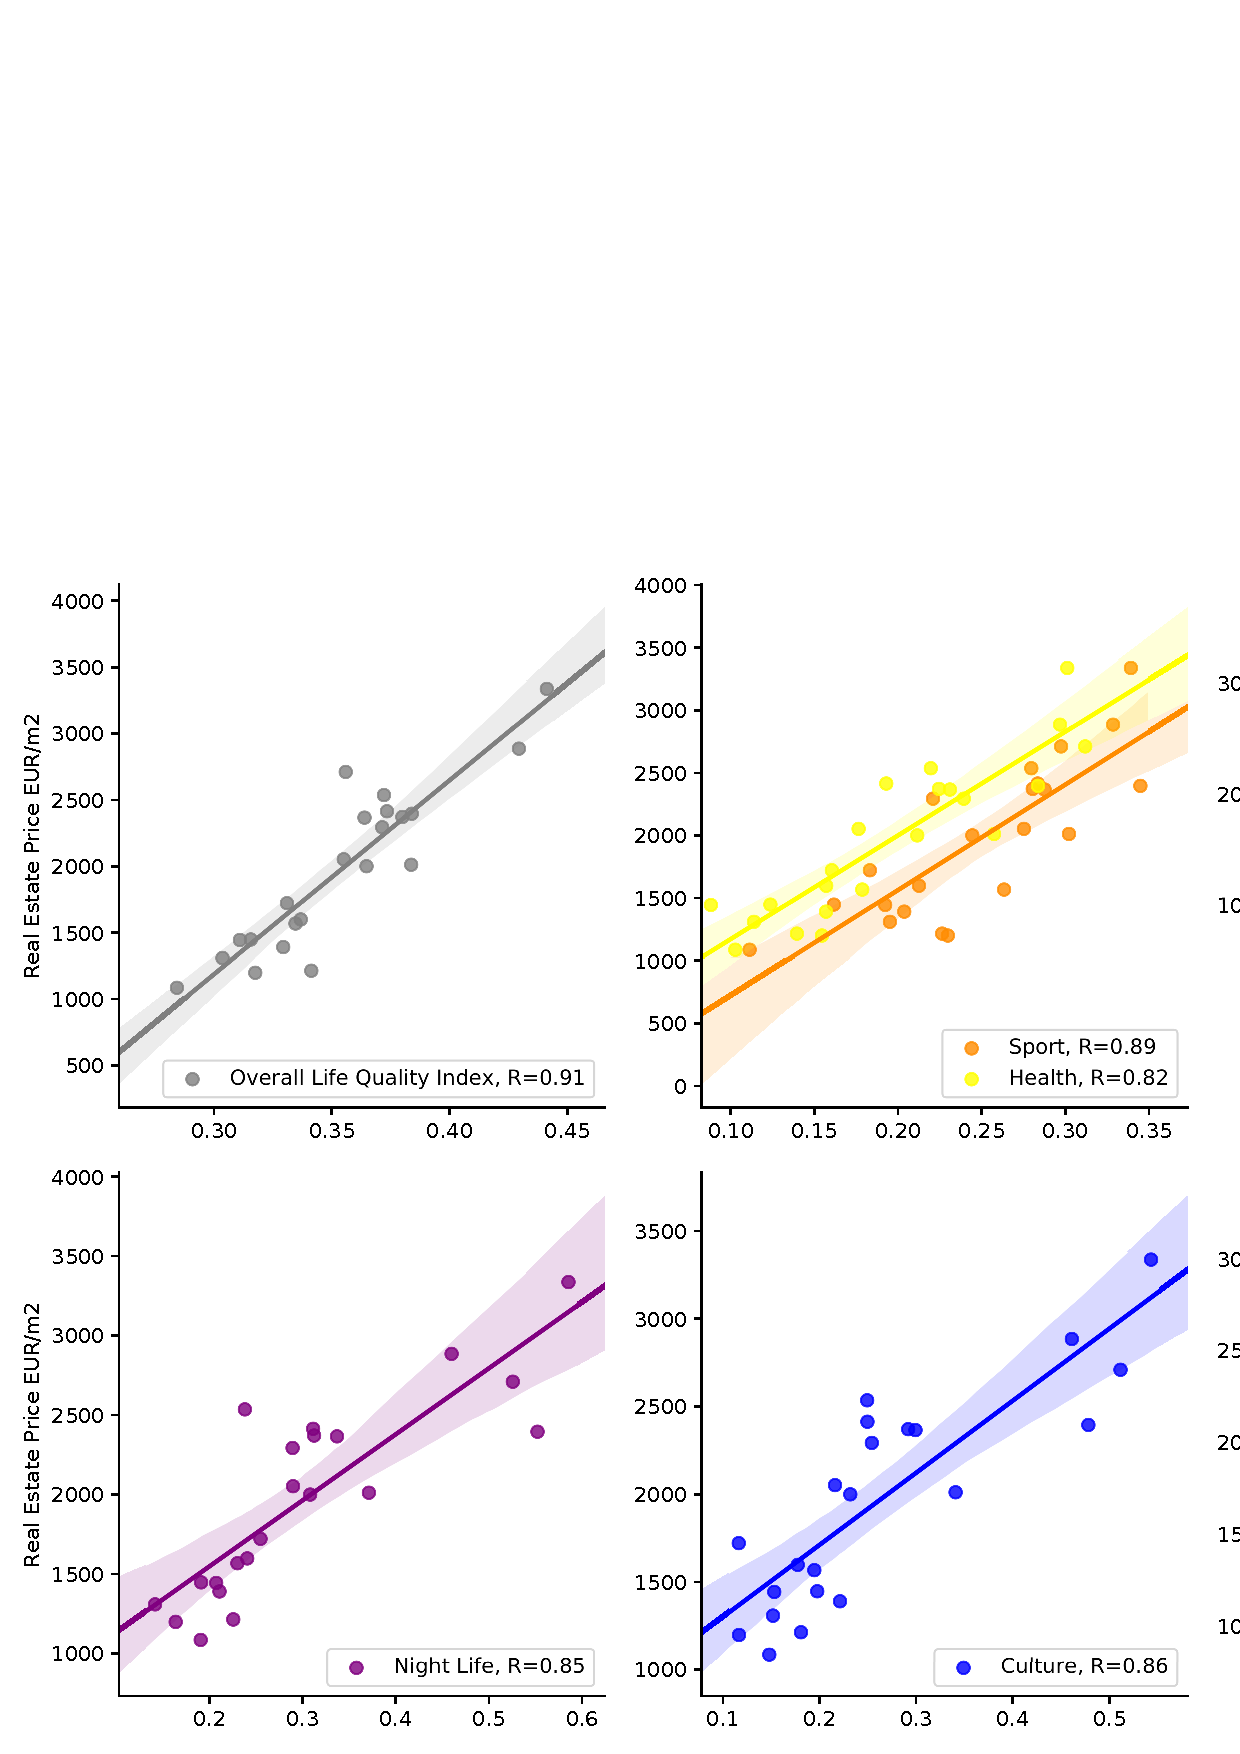
\includegraphics[width=\textwidth]{images/lqi/LQI_categories_regplots.pdf}
	\caption[Budapest life quality index correlation with real estate prices]{Districts of Budapest Life Quality Index (LQI) and its components correlated with real estate prices ($m^{2}/EUR$)}
	\label{fig:LQI_ev}
\end{figure*}

\paragraph{Summary} Locals of Budapest, like in most European cities, traditionally values downtown areas. The relative closeness to CBD, good access to public transport, and vital city life kept it as a desirable area for living~\cite{Cassiers2012Socio}. However, in recent years, the city is facing new challenges: due to gentrification~\cite{Garcia2004Cultural} and over-tourism (eg.:Airbnb) real estate prices are sky-rocketing in downtown areas. In contrast with the early 2000-s when (upper) middle-class moved to the suburbs, nowadays, lower-income families and young professionals are leaving the downtown behind in hope for more affordable living.

As our findings show, Budapest is quite centralized and the quality of life highly correlates with real estate prices, which possibly lead to even more inequalities in the future. This spatial discrimination with longer traveling time, less fulfilling environment, and potential segregation reduces the chances of upward mobility and the quality of life of individuals~\cite{Gobillon2007Mechanisms}.

\section{Discussion}
We have proposed a methodology to quantify life quality as a function of walkability on urban networks. We have used open data to capture inequalities between neighborhoods and districts in the city. We have shown that the real estate market reflects the life quality that our methods found.

A data-driven approach for quantifying life quality at such a granular level like our proposed method can help decision-makers to tackle social and environmental challenges better. Designing compact, liveable neighborhoods, considering also the upcoming environmental crisis is the number one priority of many cities worldwide.

The use of open data sources and algorithmic approaches adds up towards a systematic framework for understanding urban liveability. Our current approach is not the last word in this development since it does not yet account for multiple other variables, such as the quality of services and infrastructure, and other qualitative variables. To capture the more specific indicator of liveability in different cities it would be necessary to work with more granular and city-dependant data.

We anticipate a future stream of research focused on the use of worldwide open data sets to quantify urban liveability, including longitudinal studies in multiple cities, along with algorithmic modeling, simulations, and machine learning approaches, to first quantify the liveability, propose changes and test them with the ground truth data.
\pagestyle{fancy} %LQI walkability
\chapter{Conclusion and open questions}\label{ch:Conclusion}

This thesis set out to contribute to the characterization of multimodal transport infrastructures, develop network science data-driven methods to address the open research problem of planning and identifying strategies to improve sustainable mobility in cities. We leverage the availability of open high quality urban infrastructure data sets to build the multiplex transportation network of multiple cities, we analyze the networks first at their multiplex configuration, and later on focus our attention into the bicycle and pedestrian layers.

We started this thesis with a review on Chapter \ref{ch:litReview} of previous works on multimodal transportation and mobility research from a complex systems' perspective. 
%Talk more about what has been done and the gap to address.

We have seen that the multiplex structure of urban mobility systems has similarities between multiple cities around the world. The findings presented in Chapter \ref{ch:OverlapCensus} suggest that it is possible to identify and compare those similarities in a systematically and rigorously way using the ``overlap census'' method. These similarities produce clusters of cities with similar multimodal configurations, such as those that have lack investment in their sustainable mobility options thus having more car-centric profiles, and clusters of cities with a more balanced mobility options.

At the single layer level, we saw in Chapter \ref{ch:BikeGrowth} that a common characteristic of cities is the fragmentation of their bicycle infrastructure networks. We proposed the use of data-driven algorithms to consolidate those components into connected networks to efficiently improve sustainable transport. The two proposed algorithms, when compared with two baselines, highlight the usefulness of growing the bicycle network on a citywide scale (considering all areas of the city) rather than randomly adding bicycle infrastructure. The proposed approach is not the last word in this development, since it does not yet explicitly optimize for directness and does not account for transport flow. As pointed out, the use of data-driven algorithms to identify crucially missing links in bicycle infrastructure has the potential to improve the mobility infrastructure of cities efficiently and economically.

Finally, in Chapter \ref{ch:LQI} we presented a data-driven, network-based method to quantify the liveability of a city based on pedestrian accessibility to amenities and services. We applied the methodology to Budapest and showed that it is able to capture inequalities between neighborhoods and districts in the city. When comparing our findings to the average real state prices we found a positive correlation, the higher the quality of life, the higher the average real state prices.    Our framework demonstrates a way to leverage open data sources to evaluate the quality of life and pedestrian accessibility in systematic city-wide scale.

The three papers contribute... 
%Write contribution to the field(s)

\subsection*{Future Work}
What is next.
% The future for data-driven anti-corruption research looks bright. Data quality and access are generally improving. New sources of data will go a long way to addressing some of the shortcomings and limitations of the work in this thesis. For example, data on company owners and board members and the economic and social relations of politicians and regulators have potential to extend the scope of the work presented in this thesis. Network methods are clearly applicable in these contexts as well. For instance, by tracking social network connections of firm leaders to people in power, one could measure the extent of political corruption in a country by the effect of such connections on profitability.

% A major challenge in corruption research using big data will be to carry out causal inference. Though data collected at large scales has many advantages, for instance allowing us to observe whole markets across significant periods of time, it seems unrealistic to carry out experimental studies at the same scale, especially without the participation of government bodies. Further research is needed to extend methods of causal inference, for instance as often applied to panel data by economists, to the setting of networks.

% In the absence of causal identification, the scientific value of the methods developed in this thesis can be tested in other ways. If network analyses of procurement based risk indicators can predict corruption cases that authorities, researchers, or journalists can confirm, that would lend additional credibility to our approach. One can also strengthen the validity of these methods by finding evidence of other kinds of white-collar crime occurring among distinguished actors, following the classical adage that ``where there is smoke, there is fire''.

% The involvement of governments in anti-corruption research presents both opportunities and dangers. Public actors willing to experiment with rules or enforcement can help overcome problems of causal interpretation inherent in the study of observational data. Such collaborations also have the greatest potential for real-world impact, clearly. However, if researchers of corruption focus their attention too much on such collaborations, they would introduce a significant bias to our understanding of corruption. Indeed, where corruption is endemic, it is unlikely that relevant government bodies would be willing to participate in effective anti-corruption studies. Engagement with super-national actors with some independent authority in certain locations, for example with the World Bank in its procurement-based development projects or the EU and it cohesion funds, would overcome this issue to some extent. Certainly, the first step in this direction would be to convince individuals in these organizations of the value of network methods in the study of corruption. We hope that this thesis will be useful in this regard. 

\pagestyle{fancy} %Conclusion


\bibliographystyle{bmc-mathphys}
\bibliography{bibliography}
\chapter{Appendices}

\section{Life quality as walkability}

\subsection{Secondary data sources}
\label{SI:walkabilityData}
\begin{itemize}
  \item {Sport associations in Budapest}~\cite{HU_sport}
  \item {Kindergartens, daycares, primary and secondary education}~\cite{HU_Edu}
  \item {Art and music schools}~\cite{HU_Art}
  \item {Child health services}~\cite{HU_Child}
  \item {Social welfare system (eg.: elderly care)}~\cite{HU_Social}
  \item{Culture centers}~\cite{HU_Cult}
  \item {Indoor playgrounds}~\cite{HU_Play}
  \item{Healthcare (hospitals, private and public clinics, specialists)}~\cite{HU_Health}
  \item{Fitness and training facilities}~\cite{HU_Fitness}
  \item{Outdoor fitness facilities}~\cite{HU_outfitness}
  \item{Thermal baths and spa}~\cite{HU_Thermal}
  \item{Playgrounds and parks}~\cite{HU_Park}
\end{itemize}

\subsection{Weights used in the calculations}
The weights of the different $Q$ indices in the final aggregation as well as in sub-categories highly depends on the context and the nature of the problem. Here we present the values we used to generate the results of this study, that were agreed upon consulting with experts.\\
The weights of the sub-indices from equation (\ref{final_Q}) are of the following values:\\
$w^{services}=0.7$\\
$w^{safety}=0.1$\\
$w^{environment}=0.2$\\ \\
The category weights used in equation (\ref{Q_services}), aggregating $Q^{services}$ are:\\
$w^{family}= 0.3$;\\
$w^{health}= 0.3$;\\
$w^{culture} = 0.15$;\\
$w^{sport} = 0.15$;\\
$w^{night life}=0.1$;\\\pagestyle{fancy} %Appendices

% Change list of tables/figures to end
\listoftables
\addcontentsline{toc}{chapter}{List of Tables}

\listoffigures
\addcontentsline{toc}{chapter}{List of Figures}
% until here
\newpage
\backmatter
\afterpage{\blankpage}
\end{document}
